% Options for packages loaded elsewhere
\PassOptionsToPackage{unicode}{hyperref}
\PassOptionsToPackage{hyphens}{url}
%
\documentclass[
]{book}
\usepackage{amsmath,amssymb}
\usepackage{lmodern}
\usepackage{iftex}
\ifPDFTeX
  \usepackage[T1]{fontenc}
  \usepackage[utf8]{inputenc}
  \usepackage{textcomp} % provide euro and other symbols
\else % if luatex or xetex
  \usepackage{unicode-math}
  \defaultfontfeatures{Scale=MatchLowercase}
  \defaultfontfeatures[\rmfamily]{Ligatures=TeX,Scale=1}
\fi
% Use upquote if available, for straight quotes in verbatim environments
\IfFileExists{upquote.sty}{\usepackage{upquote}}{}
\IfFileExists{microtype.sty}{% use microtype if available
  \usepackage[]{microtype}
  \UseMicrotypeSet[protrusion]{basicmath} % disable protrusion for tt fonts
}{}
\makeatletter
\@ifundefined{KOMAClassName}{% if non-KOMA class
  \IfFileExists{parskip.sty}{%
    \usepackage{parskip}
  }{% else
    \setlength{\parindent}{0pt}
    \setlength{\parskip}{6pt plus 2pt minus 1pt}}
}{% if KOMA class
  \KOMAoptions{parskip=half}}
\makeatother
\usepackage{xcolor}
\usepackage{longtable,booktabs,array}
\usepackage{calc} % for calculating minipage widths
% Correct order of tables after \paragraph or \subparagraph
\usepackage{etoolbox}
\makeatletter
\patchcmd\longtable{\par}{\if@noskipsec\mbox{}\fi\par}{}{}
\makeatother
% Allow footnotes in longtable head/foot
\IfFileExists{footnotehyper.sty}{\usepackage{footnotehyper}}{\usepackage{footnote}}
\makesavenoteenv{longtable}
\usepackage{graphicx}
\makeatletter
\def\maxwidth{\ifdim\Gin@nat@width>\linewidth\linewidth\else\Gin@nat@width\fi}
\def\maxheight{\ifdim\Gin@nat@height>\textheight\textheight\else\Gin@nat@height\fi}
\makeatother
% Scale images if necessary, so that they will not overflow the page
% margins by default, and it is still possible to overwrite the defaults
% using explicit options in \includegraphics[width, height, ...]{}
\setkeys{Gin}{width=\maxwidth,height=\maxheight,keepaspectratio}
% Set default figure placement to htbp
\makeatletter
\def\fps@figure{htbp}
\makeatother
\setlength{\emergencystretch}{3em} % prevent overfull lines
\providecommand{\tightlist}{%
  \setlength{\itemsep}{0pt}\setlength{\parskip}{0pt}}
\setcounter{secnumdepth}{5}
\newlength{\cslhangindent}
\setlength{\cslhangindent}{1.5em}
\newlength{\csllabelwidth}
\setlength{\csllabelwidth}{3em}
\newlength{\cslentryspacingunit} % times entry-spacing
\setlength{\cslentryspacingunit}{\parskip}
\newenvironment{CSLReferences}[2] % #1 hanging-ident, #2 entry spacing
 {% don't indent paragraphs
  \setlength{\parindent}{0pt}
  % turn on hanging indent if param 1 is 1
  \ifodd #1
  \let\oldpar\par
  \def\par{\hangindent=\cslhangindent\oldpar}
  \fi
  % set entry spacing
  \setlength{\parskip}{#2\cslentryspacingunit}
 }%
 {}
\usepackage{calc}
\newcommand{\CSLBlock}[1]{#1\hfill\break}
\newcommand{\CSLLeftMargin}[1]{\parbox[t]{\csllabelwidth}{#1}}
\newcommand{\CSLRightInline}[1]{\parbox[t]{\linewidth - \csllabelwidth}{#1}\break}
\newcommand{\CSLIndent}[1]{\hspace{\cslhangindent}#1}
\usepackage{booktabs}
\usepackage{amsthm}
\makeatletter
\def\thm@space@setup{%
  \thm@preskip=8pt plus 2pt minus 4pt
  \thm@postskip=\thm@preskip
}
\makeatother
\ifLuaTeX
  \usepackage{selnolig}  % disable illegal ligatures
\fi
\usepackage[]{natbib}
\bibliographystyle{plainnat}
\IfFileExists{bookmark.sty}{\usepackage{bookmark}}{\usepackage{hyperref}}
\IfFileExists{xurl.sty}{\usepackage{xurl}}{} % add URL line breaks if available
\urlstyle{same} % disable monospaced font for URLs
\hypersetup{
  pdftitle={RMC-TotalRisk User's Guide},
  pdfauthor={C. Haden Smith and Woodrow L. Fields},
  hidelinks,
  pdfcreator={LaTeX via pandoc}}

\title{RMC-TotalRisk User's Guide}
\author{C. Haden Smith and Woodrow L. Fields}
\date{Last updated: 2025-01-12}

\begin{document}
\maketitle

{
\setcounter{tocdepth}{1}
\tableofcontents
}
\hypertarget{preface}{%
\chapter*{Preface}\label{preface}}
\addcontentsline{toc}{chapter}{Preface}

The U.S. Army Corps of Engineers TotalRisk software (RMC-TotalRisk) performs quantitative risk calculations for a system from a set of hazard, transform, system response, and consequence functions. RMC-TotalRisk is part of an integrated software suite that supports risk assessments. The software features a fully integrated modeling platform, including a modern graphical user interface, data entry, report quality charts, and diagnostic tools. RMC-TotalRisk can evaluate risk for a single component with multiple failure modes and a complex system comprised of multiple components. This document is a guide for developing a quantitative risk analysis with RMC-TotalRisk.

\hypertarget{acknowledgements}{%
\subsection*{Acknowledgements}\label{acknowledgements}}
\addcontentsline{toc}{subsection}{Acknowledgements}

RMC-TotalRisk would not exist without the support of Risk Management Center (RMC) leadership, in particular RMC Director Nathan Snorteland and Lead Engineers David Margo, Jason Needham, and Timothy O'Leary. The authors also recognize David Bowles and Ruben Jongejan for performing an external peer review of the software and risk analysis framework. The software development team is very grateful to those who contributed to the software.

\hypertarget{how-to-cite-this-guide}{%
\subsection*{How to Cite This Guide}\label{how-to-cite-this-guide}}
\addcontentsline{toc}{subsection}{How to Cite This Guide}

If you would like to cite this User's Guide, please use the following format:

\begin{citation-note}
C. H. Smith and W. L. Fields, \emph{RMC-TotalRisk user's guide}, 1st
ed.~Lakewood, CO: U.S. Army Corps of Engineers, Risk Management Center,
2025. Accessed on {\textless enter current date here\textgreater{}}.
\end{citation-note}

\hypertarget{welcome}{%
\chapter{Welcome to RMC-TotalRisk}\label{welcome}}

The U.S. Army Corps of Engineers (USACE) Risk Management Center (RMC) developed the quantitative risk analysis software (RMC-TotalRisk) to enhance and expedite risk assessments conducted by the USACE Flood Risk Management, Planning, and Dam and Levee Safety Communities of Practice.

RMC-TotalRisk is a menu-driven software that conducts risk analysis based on user-defined hazard, transform, system response, and consequence functions. The software features a fully integrated modelling platform, including a modern graphical user interface, data entry capabilities, and report quality charts and diagnostics. RMC-TotalRisk can perform multi-failure risk analysis for individual dams or levees as well as for complex system with multiple components.

\hypertarget{why-you-should-use-rmc-totalrisk}{%
\section{Why You Should Use RMC-TotalRisk}\label{why-you-should-use-rmc-totalrisk}}

RMC-TotalRisk is a powerful risk analysis software designed with an intuitive and easy-to-use interface. It simplifies the complexity of risk assessments by connecting the core components of risk --- hazard, transform, response, and consequences --- through a clear and intuitive risk diagram. The software generates a comprehensive range of risk outputs, including excess, background, total, failure, and non-failure risks. Each component of the analysis can incorporate uncertainty, and the software supports modeling multiple locations with distinct failure modes as separate system components, streamlining system-level risk evaluations.

RMC-TotalRisk offers unique capabilities that set it apart from other USACE software. It supports diverse hazard types, including floods, earthquakes, and wildfires, extending beyond the flood hazards modeled by most tools. The software also accommodates a wide range of consequence types, enabling assessments of life loss, economic impacts, and environmental effects. Seamless integration with other USACE programs allows it to import data from RMC-RFA, RMC-BestFit, RRFT, ERDC-StormSim, HEC-WAT, HEC-RAS, HEC-SSP, and LifeSim, providing unparalleled inter-software compatibility.

The software includes advanced functionalities, such as event tree analysis, which enables users to model geotechnical and structural performance with diagnostic and sensitivity tools unavailable in other USACE platforms. RMC-TotalRisk uniquely accounts for multiple failure modes, offering options for joint, competing, common cause, and mutually exclusive failure modes, each with distinct consequences. Additionally, it models dependency between failure mode capacities and hazard functions using flexible options, including user-defined correlation matrices.

RMC-TotalRisk calculates five critical types of risk --- excess, background, total, failure, and non-failure --- that are essential for informed decision-making. It provides comprehensive outputs, including loss exceedance curves, risk measures, and assurance metrics, all fully compliant with USACE policies for dam safety, levee safety, and flood risk management. Furthermore, it can replicate and update legacy risk analyses from tools like DAMRAE, LST, and HEC-FDA, enhancing its value for risk-informed investment decisions.

\hypertarget{when-you-should-use-rmc-totalrisk}{%
\section{When You Should Use RMC-TotalRisk}\label{when-you-should-use-rmc-totalrisk}}

Use RMC-TotalRisk whenever you need to perform a risk analysis, particularly when the analysis involves complex systems with multiple components, uncertainties, or dependencies. While the software is frequently applied in flood risk management, its capabilities extend far beyond this domain. RMC-TotalRisk is relevant to any scenario involving hazards, responses, and consequences, making it a versatile tool for a wide range of scientific, engineering, and policy applications.

The examples in this document relate to flood risk for dams and levees. However, the software is not limited to flood risk management applications. RMC-TotalRisk is designed as a general-purpose risk analysis software capable of estimating risk for various complex systems. Its flexibility and robust analytical framework make it suitable for applications such as:

\begin{itemize}
\item
  \textbf{Seismic Risk Assessment}: Evaluate risks associated with earthquakes, including structural vulnerabilities and potential consequences for infrastructure and populations.
\item
  \textbf{Wildfire Risk Management}: Model the spread of wildfires, estimate the probability of occurrence, and assess associated economic, environmental, and human impacts.
\item
  \textbf{Environmental Risk Analysis}: Analyze risks to ecosystems from natural or anthropogenic hazards, including climate change impacts, pollution, or habitat degradation.
\item
  \textbf{Industrial and Infrastructure Safety}: Assess risks for critical infrastructure, such as power plants, bridges, or pipelines, accounting for failure modes and interdependencies.
\item
  \textbf{Custom Applications}: Tackle any scenario where hazards and consequences can be defined, including risks related to human health, transportation systems, or supply chain disruptions.
\end{itemize}

RMC-TotalRisk's ability to integrate diverse hazards, model complex dependencies, and account for uncertainties makes it ideal for multidisciplinary applications. Whether you are working on a dam safety program, evaluating the environmental impacts of a natural disaster, or designing resilient infrastructure, RMC-TotalRisk provides the tools to comprehensively assess and communicate risk, supporting informed decision-making.

\hypertarget{risk-analysis-framework}{%
\chapter{Risk Analysis Framework}\label{risk-analysis-framework}}

In RMC-TotalRisk, a risk analysis computes the risk associated with a collection of potential failure modes for each system component. A failure mode consists of three key inputs: a hazard, the system's response to the hazard, and the consequences of that response. A non-failure mode, on the other hand, includes the hazard and the associated non-failure consequences.

A risk analysis uses four types of functions as inputs:

\begin{itemize}
\item
  \textbf{Hazard Function}: Commonly called a frequency curve, this function describes the exceedance probabilities of various hazard levels. Examples include annual maximum peak flow frequency, peak reservoir pool stage frequency, and peak ground acceleration.
\item
  \textbf{Transform Function}: This function converts hazard levels from one type to another. For example, a peak flow-frequency function can be transformed into a stage-frequency function using a flow-to-stage rating curve. Transform functions are optional.
\item
  \textbf{System Response Function}: Often referred to as a fragility curve, this function defines the conditional probability of failure for various hazard levels, such as water surface elevations (WSEs). The system response function specifies the failure mode.
\item
  \textbf{Consequence Function}: Sometimes called a damage function, this function describes the consequences of failure or non-failure for various hazard levels, such as annual maximum peak WSEs.
\end{itemize}

For example, Figure \ref{fig:figure-0} illustrates the conceptual risk analysis process for a levee with a single failure mode and a single system component. Beginning in the top left of the figure, the flood \textbf{hazard} is defined by an annual maximum peak flow-frequency distribution, estimated using flood-frequency analysis methods. Next, moving to the top right, peak flow is \textbf{transformed} to a WSE using a stage-discharge rating curve estimated using a hydraulic model. Then, moving to the bottom right, the \textbf{system response function} is defined by a probability of failure given the WSE, often derived from engineering analysis and expert elicitation methods. And finally, moving to the bottom left, the \textbf{consequences} given failure are estimated as a function of WSE.

\begin{figure}

{\centering 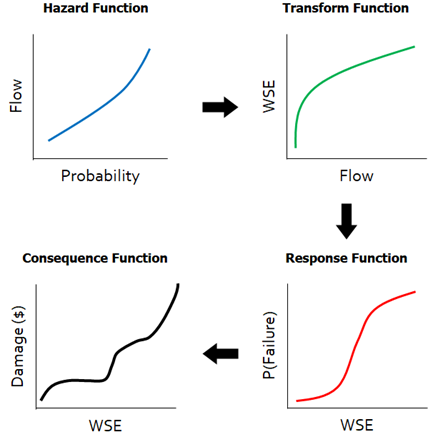
\includegraphics{images/figure0} 

}

\caption{Levee risk analysis process for a single failure mode and a single system component.}\label{fig:figure-0}
\end{figure}

The risk analysis computes the expected annual consequences by integrating over these functions. For a deeper understanding of the mathematics involved in risk analysis, refer to the technical reference manual \citep{cite-TechRef}. Additional USACE guidance on risk analysis for flood risk management is in \citep{cite-EM1619} and \citep{cite-BestPractices}.

This user guide demonstrates how to create a project; enter hazard, transform, response, and consequence functions; create a risk diagram, perform a risk analysis, and review results.

\hypertarget{installation}{%
\chapter{Installing RMC-TotalRisk}\label{installation}}

RMC-TotalRisk version 1.0 is available as a portable package (.zip). Installing a portable package does not require administrative rights. Simply extract all contents of the portable package to the desired computer location. Figure \ref{fig:figure-1} shows an example of the package contents after extraction. Double-click the executable \textbf{RMC-TotalRisk.exe} to get started. For easy access to the program, create a desktop shortcut and pin the program to the Windows task bar.

\begin{figure}

{\centering 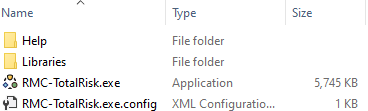
\includegraphics{images/figure1} 

}

\caption{RMC-TotalRisk executable file in the RMC-TotalRisk portable .zip directory.}\label{fig:figure-1}
\end{figure}

\hypertarget{setting-the-file-association-in-windows}{%
\section{Setting the File Association in Windows}\label{setting-the-file-association-in-windows}}

RMC-TotalRisk files have a ``.tra'' file extension. To have Windows automatically open .tra files with RMC-TotalRisk, right-click a .tra project file. Select \textbf{Open with\ldots{}} from the resulting menu (Figure \ref{fig:figure-2}).

\begin{figure}

{\centering 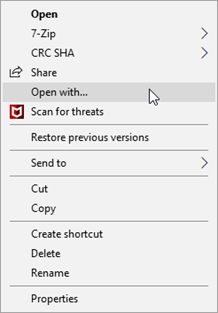
\includegraphics{images/figure2} 

}

\caption{Right-click to select how to open a file in Windows.}\label{fig:figure-2}
\end{figure}

From the menu that appears when you select \textbf{Open with\ldots{}}, click \textbf{Try an app on this PC} for an expanded list of already installed applications. If RMC-TotalRisk is not an option, scroll to the bottom and select \textbf{Look for another app on this PC}. This opens a Windows Explorer dialog. Navigate to and select the executable \textbf{RMC-TotalRisk.exe}, then click \textbf{Open}.

When you've found RMC-TotalRisk and selected it, check the box labeled \textbf{Always use this app to open {[}.tra{]} files} before you click the \textbf{OK} button. Now .tra files appear in Windows Explorer with the RMC TotalRisk icon (Figure \ref{fig:figure-3}). You can now double-click a project file to automatically open it with RMC-TotalRisk.

\begin{figure}

{\centering 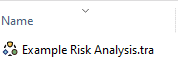
\includegraphics{images/figure3} 

}

\caption{RMC-TotalRisk project with file association in Windows.}\label{fig:figure-3}
\end{figure}

\hypertarget{system-requirements}{%
\section{System Requirements}\label{system-requirements}}

The RMC-TotalRisk program and all dependent libraries were developed using the .NET Framework 4.8.1. As such, the program is currently only available for the Microsoft Windows operating system. The recommended system configuration for RMC-TotalRisk includes:

\begin{itemize}
\item
  64-bit Windows Operating System (Windows 10 or newer).
\item
  512 MB of RAM at a minimum.
\item
  2 GB of free disk space at a minimum.
\item
  Quad-Core CPU with 2.7 GHz (or faster) clock speed.
\item
  1280 x 1024 screen resolution or higher (and at least a 17'' monitor).
\end{itemize}

\hypertarget{terms-and-conditions-for-use}{%
\section{Terms and Conditions for Use}\label{terms-and-conditions-for-use}}

The United States Government, U.S. Army Corps of Engineers, Risk Management Center (``RMC'') grants to the user the rights to install RMC-TotalRisk ``the Software'' (either from a copy obtained from RMC, a distributor or another user or by downloading it from a network) and to use, copy and/or distribute copies of the Software to other users, subject to the following Terms and Conditions of Use:

All copies of the Software received or reproduced by or for user pursuant to the authority of this Terms and Conditions of Use will be and remain the property of RMC. User may reproduce and distribute the Software provided that the recipient agrees to the Terms and Conditions for Use noted herein.

RMC is solely responsible for the content of the Software. The Software may not be modified, abridged, decompiled, disassembled, unobfuscated or reverse engineered. The user is solely responsible for the content, interactions, and effects of any and all amendments, if present, whether they be extension modules, language resource bundles, scripts or any other amendment.

The name ``RMC-TotalRisk'' must not be used to endorse or promote products derived from the Software. Products derived from the Software may not be called ``RMC-TotalRisk'' nor may any part of the ``RMC TotalRisk'' name appear within the name of derived products. No part of this Terms and Conditions for Use may be modified, deleted or obliterated from the Software. No part of the Software may be exported or re-exported in contravention of U.S. export laws or regulations.

\hypertarget{waiver-of-warranty}{%
\subsection{Waiver of Warranty}\label{waiver-of-warranty}}

THE UNITED STATES GOVERNMENT AND ITS AGENCIES, OFFICIALS, REPRESENTATIVES, AND EMPLOYEES, INCLUDING ITS CONTRACTORS AND SUPPLIERS PROVIDE RMC TOTALRISK ``AS IS,'' WITHOUT ANY WARRANTY OR CONDITION, EXPRESS, IMPLIED OR STATUTORY, AND SPECIFICALLY DISCLAIM ANY IMPLIED WARRANTIES OF TITLE, MERCHANTABILITY, FITNESS FOR A PARTICULAR PURPOSE AND NON-INFRINGEMENT. Depending on state law, the foregoing disclaimer may not apply to you, and you may also have other legal rights that vary from state to state.

\hypertarget{limitation-of-liability}{%
\subsection{Limitation of Liability}\label{limitation-of-liability}}

IN NO EVENT SHALL THE UNITED STATES GOVERNMENT AND ITS AGENCIES, OFFICIALS, REPRESENTATIVES, AND EMPLOYEES, INCLUDING ITS CONTRACTORS AND SUPPLIERS, BE LIABLE FOR LOST PROFITS OR ANY SPECIAL, INCIDENTAL OR CONSEQUENTIAL DAMAGES ARISING OUT OF OR IN CONNECTION WITH USE OF RMC-TOTALRISK REGARDLESS OF CAUSE, INCLUDING NEGLIGENCE.

THE UNITED STATES GOVERNMENT'S LIABILITY, AND THE LIABILITY OF ITS AGENCIES, OFFICIALS, REPRESENTATIVES, AND EMPLOYEES, INCLUDING ITS CONTRACTORS AND SUPPLIERS, TO YOU OR ANY THIRD PARTIES IN ANY CIRCUMSTANCE IS LIMITED TO THE REPLACEMENT OF CERTIFIED COPIES OF RMC-TOTALRISK WITH IDENTIFIED ERRORS CORRECTED. Depending on state law, the above limitation or exclusion may not apply to you.

\hypertarget{indemnity}{%
\subsection{Indemnity}\label{indemnity}}

As a voluntary user of RMC-TotalRisk you agree to indemnify and hold the United States Government, and its agencies, officials, representatives, and employees, including its contractors and suppliers, harmless from any claim or demand, including reasonable attorneys' fees, made by any third party due to or arising out of your use of RMC-TotalRisk or breach of this Agreement or your violation of any law or the rights of a third party.

\hypertarget{assent}{%
\subsection{Assent}\label{assent}}

By using this program you voluntarily accept these terms and conditions. If you do not agree to these terms and conditions, uninstall the program and return any program materials to RMC (If you downloaded the program and do not have disk media, please delete all copies, and cease using the program).

\hypertarget{gui}{%
\chapter{Graphical User Interface}\label{gui}}

RMC-TotalRisk is a menu-driven software package that performs risk analyses. The software features a fully integrated modeling platform, including a modern graphical user interface, data entry capabilities, multi-failure risk analysis, and report-quality charts.

The graphical user interface consists of a menu bar, tool bar, and four window panes (Figure \ref{fig:figure-4}): the Project Explorer, Tabbed Documents, Properties, and the Message window. You may move, dock, hide, or close the panes as desired.

\begin{figure}

{\centering 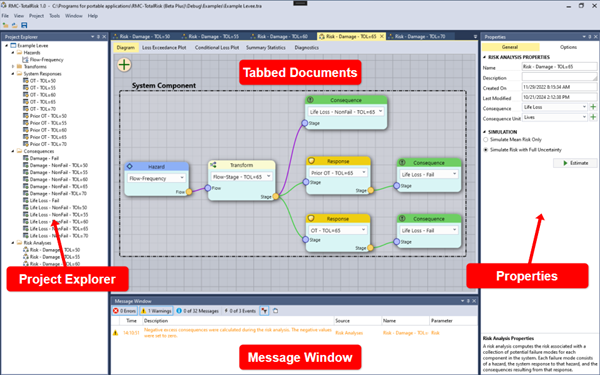
\includegraphics{images/figure4} 

}

\caption{RMC-TotalRisk graphical user interface.}\label{fig:figure-4}
\end{figure}

\hypertarget{gui-menu-bar}{%
\section{Menu Bar}\label{gui-menu-bar}}

The menu bar at the top of the window (Figure \ref{fig:figure-5}) contains important commands for working with RMC TotalRisk. The following subsections provide detail on each command.

\begin{figure}

{\centering 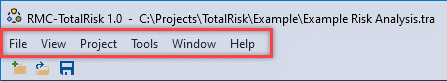
\includegraphics{images/figure5} 

}

\caption{RMC-TotalRisk menu bar.}\label{fig:figure-5}
\end{figure}

\hypertarget{gui-menu-bar-file}{%
\subsection{File}\label{gui-menu-bar-file}}

The File menu (Figure \ref{fig:figure-6}) provides essential file management functionality. From this menu, you create a new project, open an existing project, save or save as, open recent projects, or exit the application.

\begin{figure}

{\centering 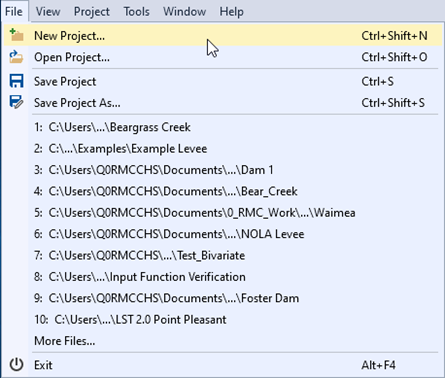
\includegraphics{images/figure6} 

}

\caption{File menu.}\label{fig:figure-6}
\end{figure}

The first time you use RMC-TotalRisk, the recent projects list will be empty. If your recent projects exceed the number that the list shows at one time (the default is 10), a menu item labeled \textbf{More Files\ldots{}} is available. That option opens a Recent Files dialog showing all available recent project files (Figure \ref{fig:figure-7}). From here, you may open any recently used project file or clear the recent project file list.

\begin{figure}

{\centering 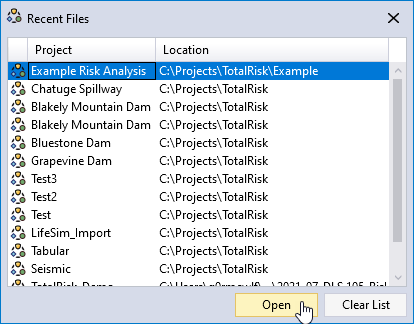
\includegraphics{images/figure7} 

}

\caption{Recent file dialog.}\label{fig:figure-7}
\end{figure}

\hypertarget{gui-menu-bar-view}{%
\subsection{View}\label{gui-menu-bar-view}}

You may move, dock, hide, or close the Project Explorer, the Properties window, and Message window as desired. The View menu (Figure \ref{fig:figure-8}) allows you to unhide or open these windows. In addition, you can restore the default layout of the panes.

\begin{figure}

{\centering 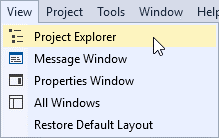
\includegraphics{images/figure8} 

}

\caption{View menu.}\label{fig:figure-8}
\end{figure}

\hypertarget{gui-menu-bar-project}{%
\subsection{Project}\label{gui-menu-bar-project}}

The Project menu (Figure \ref{fig:figure-9}) contains commands related to the project you are working in. From this menu, you can create a new hazard, transform, system response, or consequence function. You can also add a new risk analysis. In addition, you can edit the project properties through the Properties window.

\begin{figure}

{\centering 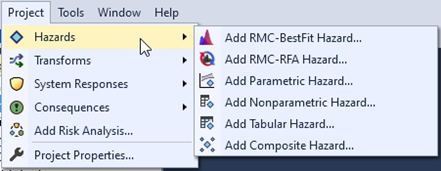
\includegraphics{images/figure9} 

}

\caption{Project menu.}\label{fig:figure-9}
\end{figure}

\hypertarget{gui-menu-bar-tools}{%
\subsection{Tools}\label{gui-menu-bar-tools}}

The Tools menu (Figure \ref{fig:figure-10}) provides tools for managing your project and personalizing your workspace.

\begin{figure}

{\centering 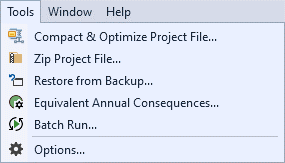
\includegraphics{images/figure10} 

}

\caption{Tools menu.}\label{fig:figure-10}
\end{figure}

\begin{itemize}
\item
  \textbf{Compact \& Optimize Project File} compacts and optimizes the project database and removes unnecessary tables. This tool can significantly reduce the size of your file without losing any project data.
\item
  \textbf{Zip Project File} zips your project file and prompts you to save the .zip to a location on your computer. The zip file is smaller and easier to share with others.
\item
  \textbf{Restore From Backup} restores the project from the backup file (***.tra.bak). Note: RMC-TotalRisk creates a backup file every 30 minutes by default. You can change the backup frequency in the Options dialog, File Management tab.
\item
  \textbf{Equivalent Annual Consequences} (Figure \ref{fig:figure-11}) calculates equivalent annual consequences (EqAC) between two risk analyses. EqAC is required in USACE cost evaluation procedures \citep{cite-TechRef}. The EqAC is automatically calculated when you define the analysis period (in years) and a discount rate (as a percentage), then select current and future risk analyses and the year those results represent. Use the table tools to add and remove EqAC calculations. You can also manually enter base and future plan results by clicking in the dropdowns and typing the value.
\end{itemize}

\begin{figure}

{\centering 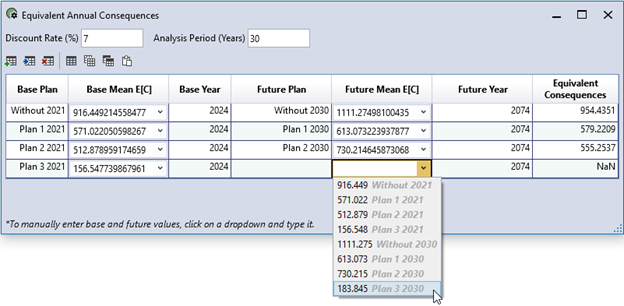
\includegraphics{images/figure11} 

}

\caption{Equaivalent Annual Consequences tool.}\label{fig:figure-11}
\end{figure}

\begin{itemize}
\tightlist
\item
  \textbf{Batch Run} (Figure \ref{fig:figure-12}) simulates multiple risk analyses as a batch process. Batch processing is very useful when inputs have been changed that are common across multiple risk analyses.
\end{itemize}

\begin{figure}

{\centering 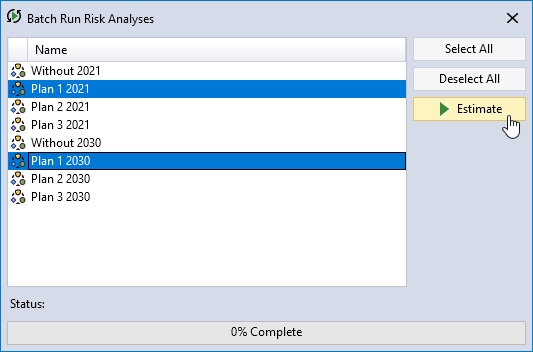
\includegraphics{images/figure12} 

}

\caption{Batch Run Risk Analyses tool.}\label{fig:figure-12}
\end{figure}

\begin{itemize}
\tightlist
\item
  \textbf{Options} lets you customize the application, file management, Message window, and default settings. See section \ref{options} for more details.
\end{itemize}

\hypertarget{gui-menu-bar-window}{%
\subsection{Window}\label{gui-menu-bar-window}}

The Window menu allows you to close or activate document windows. The active window has a check mark next to it, as shown in Figure \ref{fig:figure-13}.

\begin{figure}

{\centering 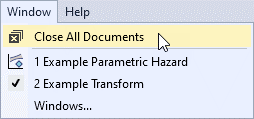
\includegraphics{images/figure13} 

}

\caption{Window menu.}\label{fig:figure-13}
\end{figure}

You can see all open windows by clicking \textbf{Windows\ldots{}}, which opens a Windows dialog (Figure \ref{fig:figure-14}). From here, you can activate or save specific document windows. In addition, you can select and close multiple windows at once.

\begin{figure}

{\centering 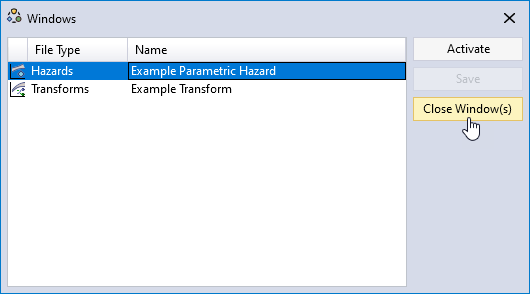
\includegraphics{images/figure14} 

}

\caption{Windows dialog.}\label{fig:figure-14}
\end{figure}

\hypertarget{gui-menu-bar-help}{%
\subsection{Help}\label{gui-menu-bar-help}}

From the Help menu, you can access this User's Guide (Figure \ref{fig:figure-15}), view the Terms and Conditions for Use, or view the About RMC-TotalRisk splash screen (Figure \ref{fig:figure-16}).

\begin{figure}

{\centering 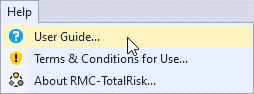
\includegraphics{images/figure15} 

}

\caption{Help menu.}\label{fig:figure-15}
\end{figure}

\begin{figure}

{\centering 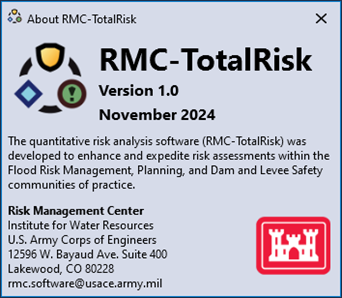
\includegraphics{images/figure16} 

}

\caption{About RMC-TotalRisk splash screen.}\label{fig:figure-16}
\end{figure}

\hypertarget{gui-tool-bar}{%
\section{Tool Bar}\label{gui-tool-bar}}

The Tool Bar is on the main window, below the Menu Bar, with buttons for frequently used options under the File menu: New Project, Open Project, and Save Project (Figure \ref{fig:figure-17}).

\begin{figure}

{\centering 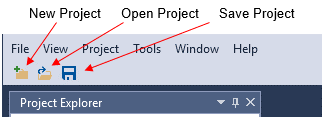
\includegraphics{images/figure17} 

}

\caption{RMC-TotalRisk tool bar.}\label{fig:figure-17}
\end{figure}

\hypertarget{gui-window-layout}{%
\section{Window Layout}\label{gui-window-layout}}

In RMC-TotalRisk, you can customize the position, size, and behavior of windows to create layouts that work best for you. When you customize the layout, RMC-TotalRisk remembers the configuration. For example, if you change the docking location of the Project Explorer and then close RMC-TotalRisk, the next time that you open the software, the Project Explorer is docked in that same location.

\hypertarget{types-of-windows}{%
\subsection{Types of Windows}\label{types-of-windows}}

RMC-TotalRisk has four basic window types: the Project Explorer, Tabbed Documents, Properties, and the Message Window (Figure \ref{fig:figure-4}). These windows provide editing and reviewing space for the various project components, including hazard, response, and consequence functions. For tool windows, resize and drag them by their title bars. For document windows, drag them by their tabs.

On the title bars in the Project Explorer, Properties window, and Message Window, a dropdown offers other options (Figure \ref{fig:figure-18}).

\begin{figure}

{\centering 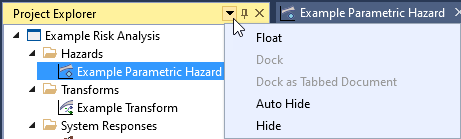
\includegraphics{images/figure18} 

}

\caption{Tools window options.}\label{fig:figure-18}
\end{figure}

On the Tabbed Documents pane, you can right-click on document tabs to set other options on the window. These options include docking, floating, and hiding windows (Figure \ref{fig:figure-19}).

\begin{figure}

{\centering 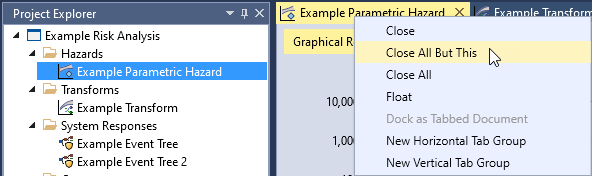
\includegraphics{images/figure19} 

}

\caption{Document window options.}\label{fig:figure-19}
\end{figure}

\hypertarget{tab-groups}{%
\subsection{Tab Groups}\label{tab-groups}}

When you are working with two or more open documents in RMC-TotalRisk, you can group tabbed documents to enhance your ability to manage a limited workspace. Organize multiple document and tool windows into either vertical or horizontal tab groups or move documents from one group to another by dragging and dropping them; even float and move windows and tab groups to different monitors. When you need to view or edit two documents at once, you can split windows by creating two horizontal tab groups, as shown in Figure \ref{fig:figure-20}.

\begin{figure}

{\centering 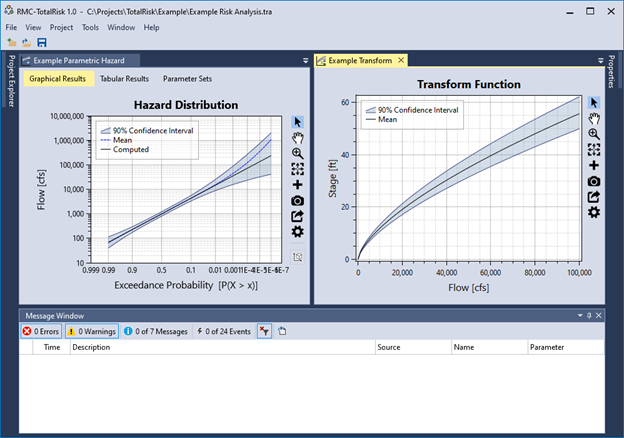
\includegraphics{images/figure20} 

}

\caption{Split document windows.}\label{fig:figure-20}
\end{figure}

\hypertarget{move-and-dock-windows}{%
\subsection{Move and Dock Windows}\label{move-and-dock-windows}}

You can dock a document window in the Tabbed Documents area or float it as a separate window independent of the main window. You can arrange windows in the following ways:

\begin{itemize}
\item
  Dock tool windows to the edge of the main window frame.
\item
  Float tool and document windows over or outside the main window.
\item
  Hide tool windows along the edge of the main window.
\item
  Display windows on different monitors.
\item
  Reset window placement to the default layout by choosing \textbf{View \textgreater{} Reset Default Layout}.
\end{itemize}

Arrange windows by dragging or right-clicking the title bar or tab of the window being arranged. When you click and drag the title bar of a tool window or the tab of a document window, a cross-shaped window placement guide appears. During the drag operation, when the cursor is over one of the arrows in the guide, a shaded area appears that shows you where the window docks if you release the mouse button. Figure \ref{fig:figure-21} and Figure \ref{fig:figure-22} show examples of the window placement guide.

\begin{figure}

{\centering 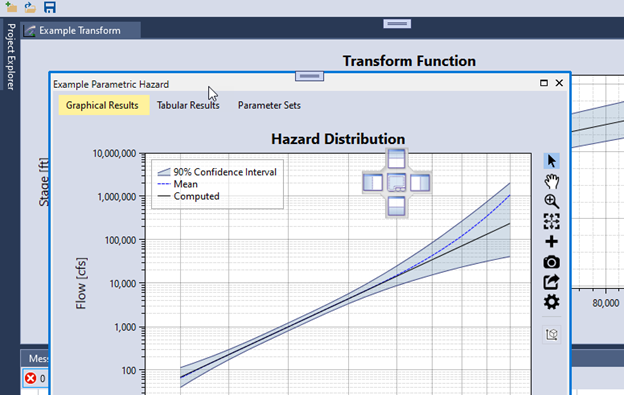
\includegraphics{images/figure21} 

}

\caption{Moving and docking document windows.}\label{fig:figure-21}
\end{figure}

Figure 22 shows the Properties window being docked below the Project Explorer. The new location is demarcated by the light blue shared area.

\begin{figure}

{\centering 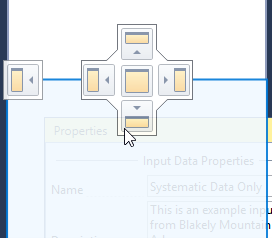
\includegraphics{images/figure22} 

}

\caption{Example of docking the Properties window below the Project Explorer.}\label{fig:figure-22}
\end{figure}

\hypertarget{close-and-auto-hide-tool-windows}{%
\subsection{Close and Auto-Hide Tool Windows}\label{close-and-auto-hide-tool-windows}}

You can close a tool window by clicking on the X in the upper right of the title bar. To reopen the tool window, navigate to the View menu and select the desired tool window to show. Tool windows have an auto-hide feature, which causes a window to slide out of the way when you use a different window. When a window is auto-hidden, the window name appears on the tab at the edge of the main window, as shown in Figure \ref{fig:figure-23}. To show the window again, move your mouse cursor over the tab and the window slides back into view.

\begin{figure}

{\centering 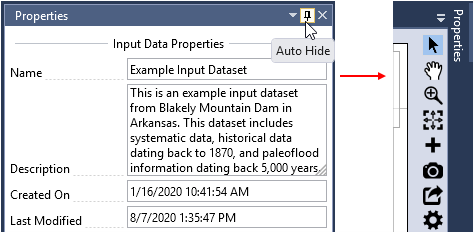
\includegraphics{images/figure23} 

}

\caption{Auto-Hide tool window.}\label{fig:figure-23}
\end{figure}

\hypertarget{project-explorer}{%
\section{Project Explorer}\label{project-explorer}}

The Project Explorer* which is typically on the left-hand side of the main window, shows a graphical representation of the hierarchy of elements within your project (Figure \ref{fig:figure-24}). After you create a new project, you can use the Project Explorer to view, navigate, and manage the project elements.

\begin{figure}

{\centering 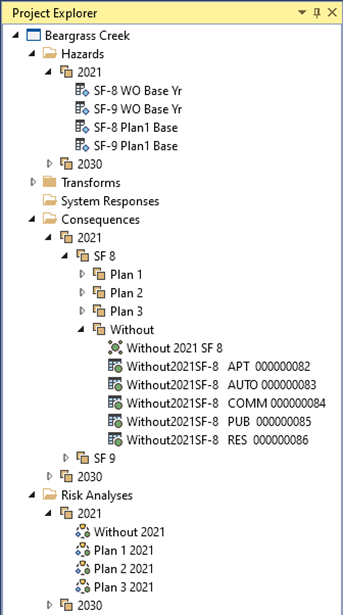
\includegraphics{images/figure24} 

}

\caption{Project Explorer.}\label{fig:figure-24}
\end{figure}

Project elements are organized under folder headers: Hazards, Transforms, System Responses, Consequences, and Risk Analyses.

Many menu commands are available by right-clicking on various items in the Project Explorer. You can create new elements, create groups, or sort the items in each folder by right-clicking the folder icon or name (Figure \ref{fig:figure-25}).

\begin{figure}

{\centering 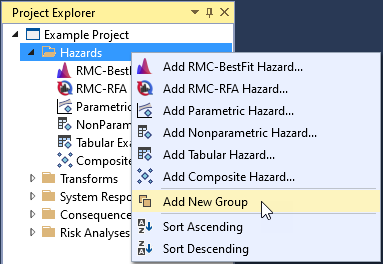
\includegraphics{images/figure25} 

}

\caption{Example of a menu available by right-clicking on a Project Explorer folder header.}\label{fig:figure-25}
\end{figure}

When right-clicking an individual project element, the following commands are available: Edit, Copy, Rename, Delete, Move Up, and Move Down (Figure \ref{fig:figure-26}, left side). When multiple project elements are selected, three right-click menu commands are available: Group, Edit, and Delete (Figure \ref{fig:figure-26}, right side). Double-clicking a project element opens it for editing.

\begin{figure}

{\centering 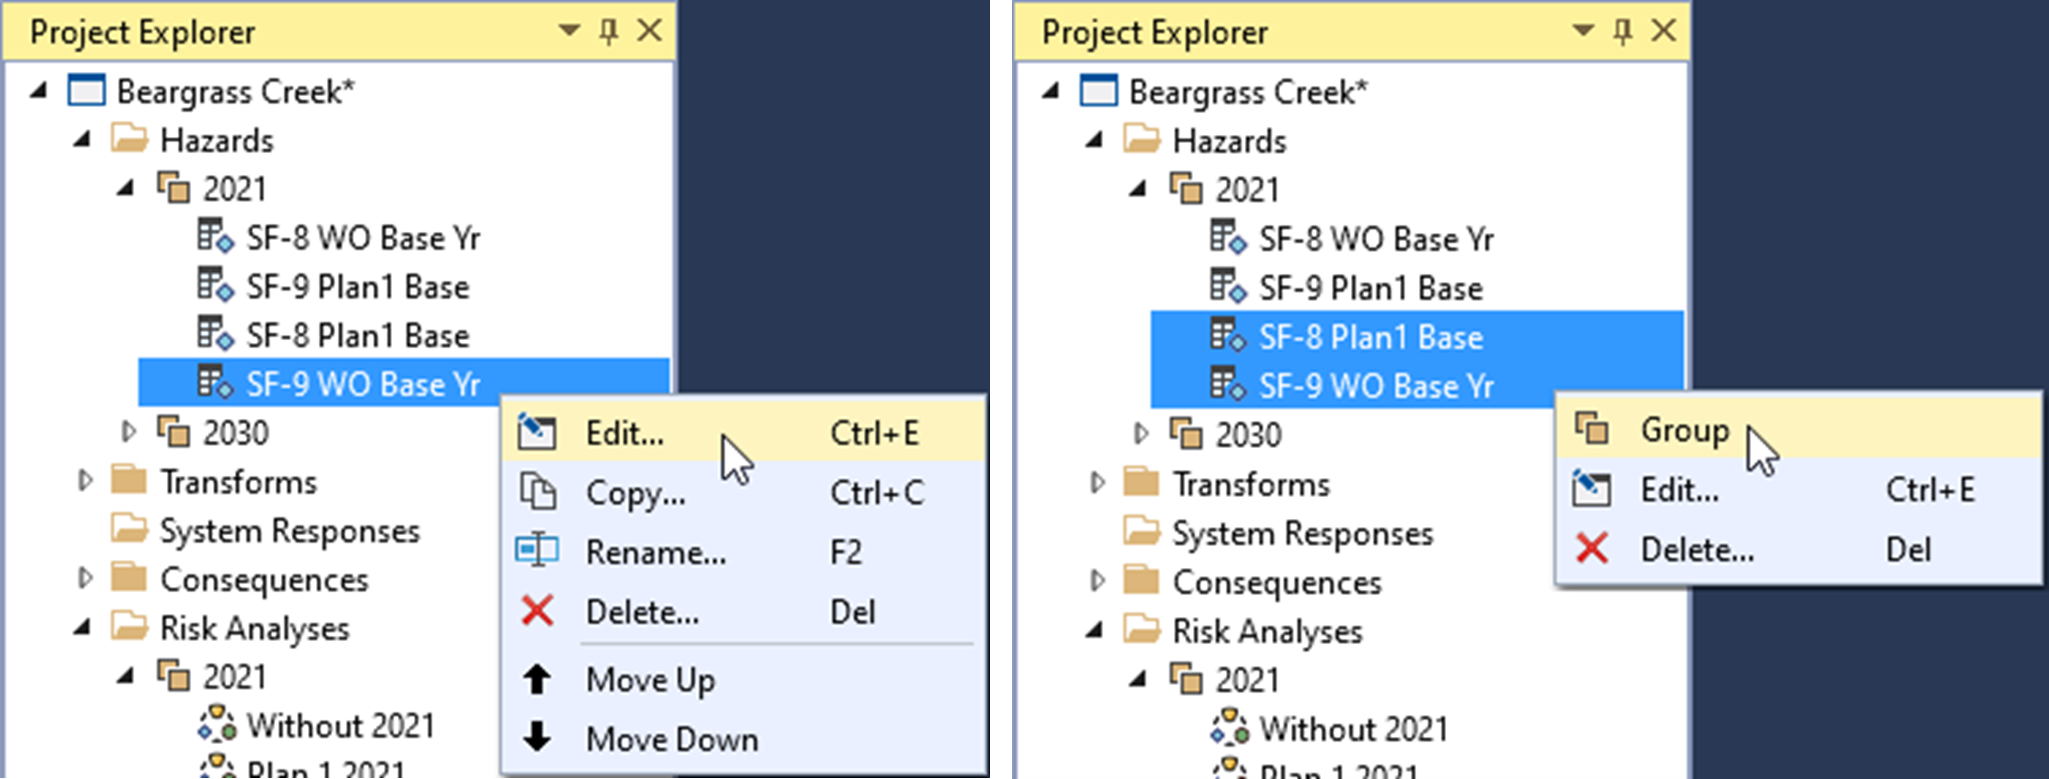
\includegraphics{images/figure26} 

}

\caption{Examples of menu options available by right-clicking on project elements: for a single selection (left) or multiple selections (right).}\label{fig:figure-26}
\end{figure}

You can move individual project elements by left-clicking, holding, and dragging the element. A horizontal line indicates where the element will move to (Figure \ref{fig:figure-27}). You can also drag and drop input data from one RMC-TotalRisk project to another.

\begin{figure}

{\centering 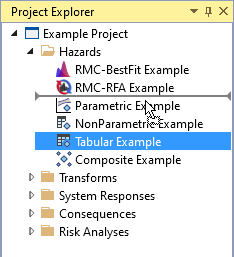
\includegraphics{images/figure27} 

}

\caption{Project Explorer element drag and drop.}\label{fig:figure-27}
\end{figure}

Grouping provides a way to manage the Project Explorer by consolidating project elements into subgroups. When right-clicking a group element, all commands from the root folder are available, as well as Ungroup and Rename (Figure \ref{fig:figure-28}).

\begin{figure}

{\centering 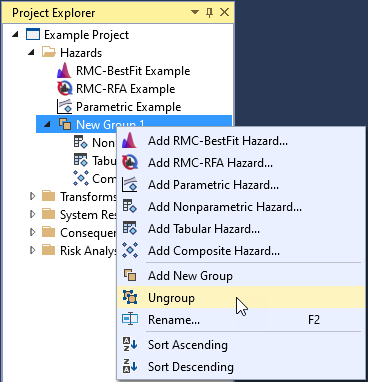
\includegraphics{images/figure28} 

}

\caption{Project Explorer group elements.}\label{fig:figure-28}
\end{figure}

\hypertarget{tabbed-documents}{%
\section{Tabbed Documents}\label{tabbed-documents}}

In RMC-TotalRisk, document windows contain the project element data, such as input tabular data, event trees, and risk analyses. Opening a project element for editing automatically opens the Tabbed Document pane, which is typically in the center of the main window (see Figure \ref{fig:figure-29}). You can reorder the tabbed documents or drag or float them outside of the main window. When you click on, or activate, a document window, the Properties window shows the associated project element properties.

\begin{figure}

{\centering 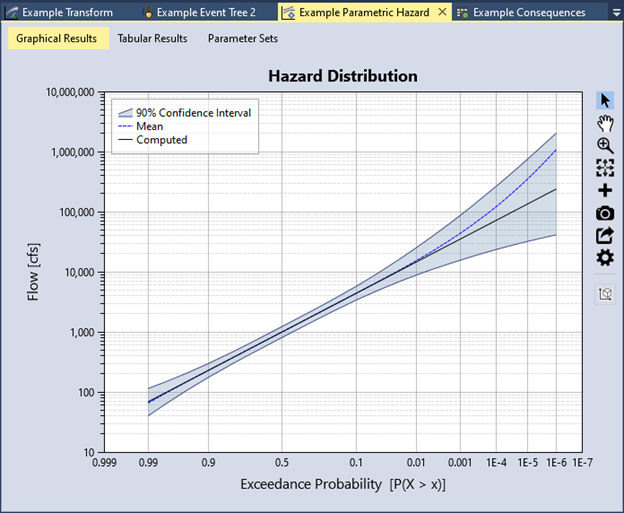
\includegraphics{images/figure29} 

}

\caption{Tabbed Document pane.}\label{fig:figure-29}
\end{figure}

\hypertarget{properties-window}{%
\section{Properties Window}\label{properties-window}}

The Properties window, typically on the right-hand side of the main window, displays the properties for the project and selected project elements. To access the element properties, open the element for edit. Some properties are common to all project elements, such as name and description, while others are unique to the specific elements. Properties are organized into groups for easier navigation. When you click on a property, the property description displays at the bottom of the Properties window, as shown in Figure \ref{fig:figure-30}. All analyses run from the Properties window.

\begin{figure}

{\centering 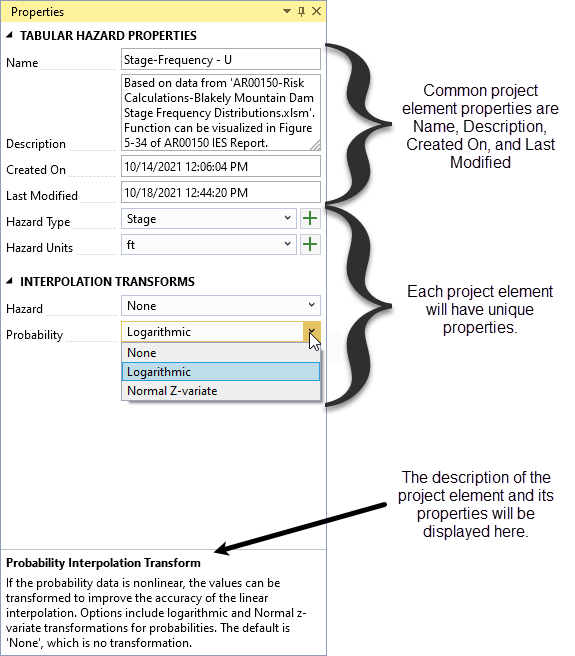
\includegraphics{images/figure30} 

}

\caption{Properties window.}\label{fig:figure-30}
\end{figure}

\hypertarget{message-window}{%
\section{Message Window}\label{message-window}}

The Message window (Figure \ref{fig:figure-31}) shows you errors, warnings, messages, and event logs regarding the current state of your project. If your project file has any errors, they are listed here. The Message window lets you perform the following tasks:

\begin{itemize}
\item
  Display the errors, warnings, messages, and events produced while you work in RMC-TotalRisk.
\item
  Double-click any error message entry to open the project element where the problem occurs.
\item
  Filter the types of entries that the Message window displays by clicking on the tabs. The default is to only display errors and warnings.
\item
  Export all entries to a text file.
\end{itemize}

Once you resolve an error, warning, or message, the entry disappears from the Message window. You may customize the font color of the various message types by navigating to \textbf{Tools \textgreater{} Options}. See section \ref{options} for more details.

\begin{figure}

{\centering 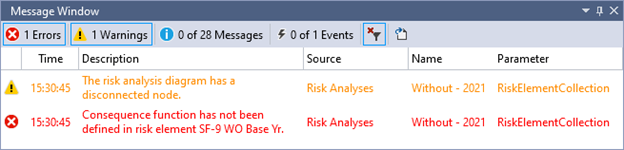
\includegraphics{images/figure31} 

}

\caption{Message window.}\label{fig:figure-31}
\end{figure}

\hypertarget{options}{%
\section{Personalize RMC-TotalRisk}\label{options}}

You can personalize RMC-TotalRisk in various ways to enhance the user experience by navigating to \textbf{Tools \textgreater{} Options}. The Options dialog allows you to customize the application, file management, Message Window, and default settings.

\hypertarget{application-options}{%
\subsection{Application Options}\label{application-options}}

You can set the application color theme to the Light or Blue theme, as shown in Figure \ref{fig:figure-32} and Figure \ref{fig:figure-33}. The default is the Light theme. If you select \textbf{Save the window docking layout on close}, RMC-TotalRisk remembers it when you reopen the application. You can also set the number of window items in the Window menu and the number of recent project items in the Recent Project list under the File menu.

\begin{figure}

{\centering 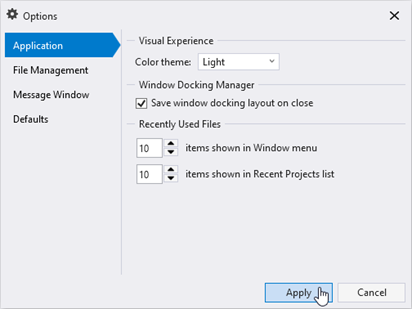
\includegraphics{images/figure32} 

}

\caption{Options dialog with light color theme.}\label{fig:figure-32}
\end{figure}

\begin{figure}

{\centering 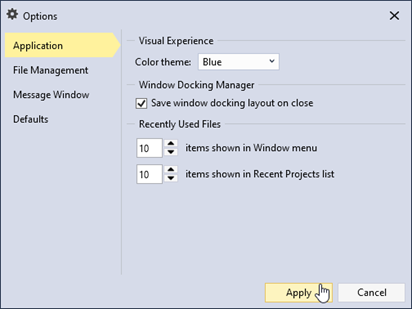
\includegraphics{images/figure33} 

}

\caption{Options dialog with blue color theme.}\label{fig:figure-33}
\end{figure}

\hypertarget{file-management-options}{%
\subsection{File Management Options}\label{file-management-options}}

RMC-TotalRisk project files are saved as SQLite databases. \href{https://www.sqlite.org/}{SQLite} is a self-contained, high-reliability, SQL database engine, which is also one of the most used database engines in the world. Database files can grow quickly as you use them, sometimes hindering performance. They can also occasionally become corrupt or damaged. Under Tools, select \textbf{Compact \& Optimize Project File} to prevent or fix these problems. You can also set RMC-TotalRisk to \textbf{Compact \& optimize project file on close} by checking the checkbox.

You can set the time interval in which a project backup file is created (Figure \ref{fig:figure-34}). A file with the extension .bak is automatically created when a project is opened. If the project closes successfully, then the .bak file is deleted. On occasion, if the database file is damaged or corrupted, or the system closes unexpectedly causing you to lose important data, you might need to restore the project from a backup file by selecting \textbf{Tools \textgreater{} Restore from Backup} (Figure \ref{fig:figure-35}).

\begin{figure}

{\centering 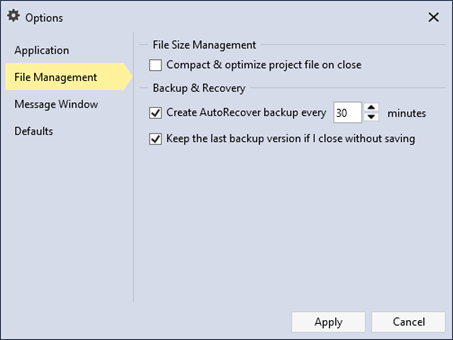
\includegraphics{images/figure34} 

}

\caption{File management options.}\label{fig:figure-34}
\end{figure}

\begin{figure}

{\centering 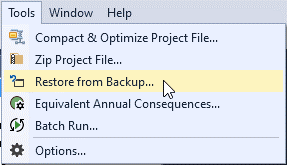
\includegraphics{images/figure35} 

}

\caption{Restore from backup.}\label{fig:figure-35}
\end{figure}

\hypertarget{message-window-options}{%
\subsection{Message Window Options}\label{message-window-options}}

You can adjust the auditory and visual settings for the Message window. You can turn message beeps on or off and select the font color for the different message types, as shown in Figure \ref{fig:figure-36}.

\begin{figure}

{\centering 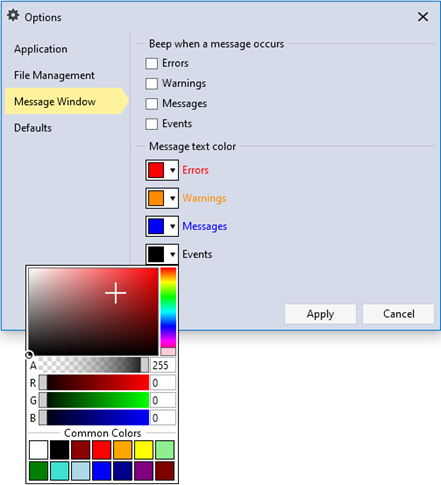
\includegraphics{images/figure36} 

}

\caption{Message window options.}\label{fig:figure-36}
\end{figure}

\hypertarget{default-options}{%
\subsection{Default Options}\label{default-options}}

You can set the default project location directory and the default number of decimal digits for the project inputs and outputs (Figure \ref{fig:figure-37}). In addition, you can set the default hazard type and units for each input function category. For example, by default, when you create a new hazard function, the hazard type and unit are automatically set to Stage and ft, respectively.

If the desired hazard type or unit is missing, click the ``plus'' button to add a new option. If you want to delete an option, click the \textbf{X} that appears by that option inside the dropdown.

\begin{figure}

{\centering 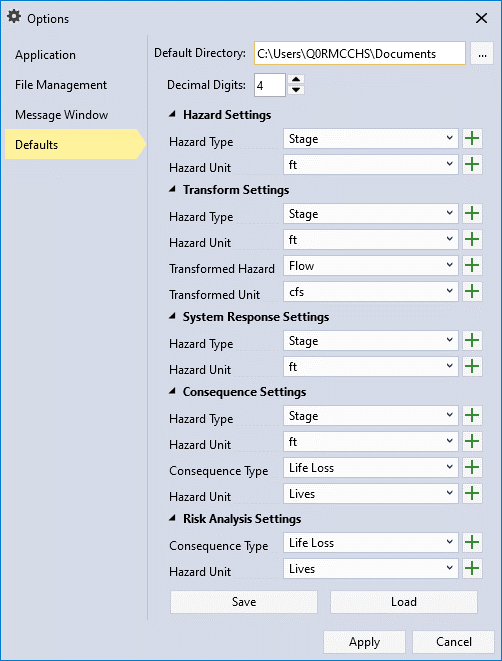
\includegraphics{images/figure37} 

}

\caption{Default options.}\label{fig:figure-37}
\end{figure}

\hypertarget{plot-features}{%
\section{Plot Features}\label{plot-features}}

RMC-TotalRisk's plot features help you examine and customize the plots. Each plot has a toolbar to the right that lets you to interact with the plot in various ways (Figure \ref{fig:figure-38}).

\begin{figure}

{\centering 
\includegraphics{images/figure38} 

}

\caption{RMC-TotalRisk plot feature icons.}\label{fig:figure-38}
\end{figure}

\begin{itemize}
\tightlist
\item
  
\includegraphics{images/trackdata.png} \textbf{Track Data} by clicking on any plotted point or line in the graph. A tooltip then displays the plot series name along with the X and Y data points (Figure \ref{fig:figure-39}).
\end{itemize}

\begin{figure}

{\centering 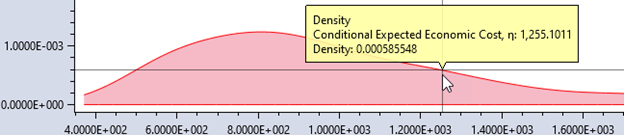
\includegraphics{images/figure39} 

}

\caption{Using Track Data on a plot.}\label{fig:figure-39}
\end{figure}

\begin{itemize}
\item
  
\includegraphics{images/pan.png} \textbf{Pan} the plot area by clicking, holding, and dragging the graph with your mouse. You can pan in any direction: up, down, or side to side. Alternatively, use the middle mouse button to pan by clicking, holding, and dragging.
\item
  
\includegraphics{images/zoomin.png} \textbf{Zoom In} by clicking, holding, and dragging with your mouse to highlight the area of interest with the magnifying glass cursor (Figure \ref{fig:figure-40}) You can also zoom in on a single axis by clicking, holding, and dragging along that axis. Alternatively, use the mouse wheel to zoom in or out.
\end{itemize}

\begin{figure}

{\centering 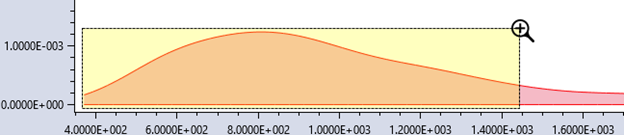
\includegraphics{images/figure40} 

}

\caption{Zooming in on a plot.}\label{fig:figure-40}
\end{figure}

\begin{itemize}
\item
  
\includegraphics{images/zoomout.png} \textbf{Zoom Out} to return to the full plot extents. You can also press the Escape key to zoom out.
\item
  
\includegraphics{images/annotations.png} \textbf{Add Annotations} to the plot to provide additional information not included in a plot series. You can choose from the following annotation types: arrow, text, vertical line, horizontal line, rectangle, ellipse, point, polygon, and polyline (Figure \ref{fig:figure-41}). Note: Legends cannot be annotated, and you cannot use annotations with the tracker.
\end{itemize}

\begin{figure}

{\centering 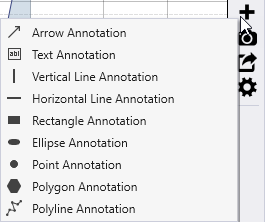
\includegraphics{images/figure41} 

}

\caption{Available plot annotations.}\label{fig:figure-41}
\end{figure}

\begin{itemize}
\tightlist
\item
  Move annotations by clicking and dragging them to a new position. Figure \ref{fig:figure-42} shows an example of an arrow and horizontal line annotation. You can edit the default annotation text by right-clicking on the annotation or through the plot properties window.
\end{itemize}

\begin{figure}

{\centering 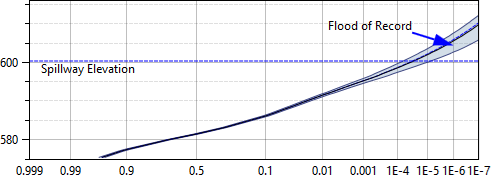
\includegraphics{images/figure42} 

}

\caption{Example of plot annotations.}\label{fig:figure-42}
\end{figure}

\begin{itemize}
\tightlist
\item
  
\includegraphics{images/saveplot.png} \textbf{Save} plot images as PNG, PDF, or SVG files. Choose from common image sizes or define your own dimensions (Figure \ref{fig:figure-43}).
\end{itemize}

\begin{figure}

{\centering 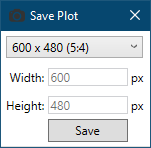
\includegraphics{images/figure43} 

}

\caption{Set the width and height of the plot image.}\label{fig:figure-43}
\end{figure}

\begin{itemize}
\item
  \includegraphics{images/exportplot.png} \textbf{Export} plot series data to a Comma Separate (.csv), Microsoft Excel® (.xlsx), or SQLite (.sqlite) file. Click the \textbf{Export Series Data} button to open a Save As dialog. Choose the file type, enter a name, and click \textbf{Save}. If you export to an existing Excel file, RMC-TotalRisk saves the plot series data as new tabs in that file.
\item
  \includegraphics{images/plotproperties.png} \textbf{Edit Plot Properties} to customize the plot's appearance (Figure \ref{fig:figure-44}). In the Properties window, adjust general plot settings, legends, axes, series, and annotations. Use the dropdown in the upper-right corner to access other plot elements for editing. RMC-TotalRisk saves plot changes and applies them when you reopen the project.
\end{itemize}

\begin{figure}

{\centering \includegraphics{images/figure44} 

}

\caption{Plot properties.}\label{fig:figure-44}
\end{figure}

\hypertarget{table-features}{%
\section{Table Features}\label{table-features}}

Tables in RMC-TotalRisk include versatile tools for adding and removing rows, exporting and copying data, and selecting rows. The following subsections describe these table features and tools in detail.

\hypertarget{add-and-remove-row-tools}{%
\subsection{Add and Remove Row Tools}\label{add-and-remove-row-tools}}

\begin{itemize}
\item
  \includegraphics{images/addrow.png} \textbf{Add Row}: Adds a row to the bottom of the table.
\item
  \includegraphics{images/insertrow.png} \textbf{Insert Row}: Inserts a row above the selected cell(s).
\item
  \includegraphics{images/deleterow.png} \textbf{Delete Row}: Deletes the row(s) containing the selected cell(s).
\end{itemize}

\hypertarget{export-and-copy-tools}{%
\subsection{Export and Copy Tools}\label{export-and-copy-tools}}

\begin{itemize}
\item
  \includegraphics{images/selectallcells.png} \textbf{Select All Cells}: Selects all cells in the table.
\item
  \includegraphics{images/copyselectedcells.png} \textbf{Copy Selected Cells}: Copies the currently selected cells to the clipboard for pasting into other applications (e.g., Microsoft Excel).
\item
  \includegraphics{images/copywheaders.png} \textbf{Copy Selected Cells with Table Headers}: Copies the selected cells along with their headers for use in other applications.
\item
  \includegraphics{images/tablepaste.png} \textbf{Paste from Clipboard into Table}: Pastes data from another table or application into the current table.
\item
  \includegraphics{images/exporttable.png} \textbf{Export Table}: Available for output tables only. Opens a Save As dialog to export the table in various formats, including Microsoft Excel (.xlsx). If you choose an existing Excel file, the table will be added as a new tab.
\end{itemize}

\hypertarget{table-row-selection-tools}{%
\subsection{Table Row Selection Tools}\label{table-row-selection-tools}}

Row selection tools are exclusive to output tables.

\begin{itemize}
\tightlist
\item
  \includegraphics{images/selectbyattribute.png} \textbf{Select Rows By Attribute}. Opens the Select By Attribute dialog box (Figure \ref{fig:figure-45}), allowing you to perform queries, make selections, and locate features in the table.
\end{itemize}

\begin{figure}

{\centering \includegraphics{images/figure45} 

}

\caption{Select By Attribute dialog.}\label{fig:figure-45}
\end{figure}

\begin{itemize}
\item
  \includegraphics{images/showallrows.png} \textbf{Show All Rows}: Displays all rows in the table after an attribute-based selection. Selected rows are highlighted in blue.
\item
  \includegraphics{images/showselectedrows.png} \textbf{Show Selected Rows Only}: Displays only the rows selected by the attribute-based query.
\item
  \includegraphics{images/deselectrows.png} \textbf{Deselect All Rows}: Clears all row selections.
\end{itemize}

\hypertarget{table-column-features}{%
\subsection{Table Column Features}\label{table-column-features}}

\begin{itemize}
\tightlist
\item
  \textbf{Sort and Search}: Sort and search table columns. For numeric values in output tables, you can also generate summary statistics (Figure \ref{fig:figure-46}). Sort by right-clicking on a column header and selecting the desired sort option or by double clicking on the column header to sort. Note: Double-clicking a column header that is already sorted sorts it in the opposite order.
\end{itemize}

\begin{figure}

{\centering \includegraphics{images/figure46} 

}

\caption{Table column header right-click options.}\label{fig:figure-46}
\end{figure}

\begin{itemize}
\tightlist
\item
  \textbf{Summary Statistics}: Use this tool to view detailed statistics for a column's data. To calculate statistics for specific rows, check the \textbf{Selected Rows Only} box (e.g., rows where the System Response Probability (SRP) exceeds the 25th percentile) (Figure \ref{fig:figure-47}).
\end{itemize}

\begin{figure}

{\centering \includegraphics[width=0.85\linewidth]{images/figure47} 

}

\caption{Table column header right-click options.}\label{fig:figure-47}
\end{figure}

\hypertarget{create-a-project}{%
\chapter{Create a Project}\label{create-a-project}}

When you open RMC-TotalRisk, it automatically creates a Blank Project file, as shown in Figure \ref{fig:figure-48}. The blank project is stored in your local temp directory. You may begin working with the blank project file immediately.

\begin{figure}

{\centering \includegraphics{images/figure48} 

}

\caption{RMC-TotalRisk blank project.}\label{fig:figure-48}
\end{figure}

To save changes to the blank project, click the Save button on the tool bar or under the \textbf{File} menu. This opens the \textbf{Save Project As\ldots{}} prompt (Figure \ref{fig:figure-49}). Enter the desired file name and click the save button in the bottom right. Now you are ready to continue working with RMC-TotalRisk.

\begin{figure}

{\centering \includegraphics{images/figure49} 

}

\caption{Save project as....}\label{fig:figure-49}
\end{figure}

You can also create a new project by clicking \textbf{New Project\ldots{}} under the \textbf{File} menu (Figure \ref{fig:figure-50}) or by clicking the \textbf{New Project} button on the tool bar (Figure \ref{fig:figure-51}). The first time you use RMC TotalRisk, the recent projects list will be empty.

\begin{figure}

{\centering \includegraphics{images/figure50} 

}

\caption{Crete new project from the file menu.}\label{fig:figure-50}
\end{figure}

\begin{figure}

{\centering \includegraphics{images/figure51} 

}

\caption{Crete new project from the tool bar.}\label{fig:figure-51}
\end{figure}

The project properties are shown in the \textbf{Properties} window (Figure \ref{fig:figure-52}), which is typically on the right hand side of the main window. You may edit the project name and description.

\begin{figure}

{\centering \includegraphics{images/figure52} 

}

\caption{Project properties.}\label{fig:figure-52}
\end{figure}

\hypertarget{hazard-functions}{%
\chapter{Hazard Functions}\label{hazard-functions}}

RMC-TotalRisk defines a hazard function by the exceedance probabilities of various hazard levels, such as annual maximum peak flow or WSE. Hazard functions are also commonly referred to as frequency curves. In dam and levee risk assessments, the annual maximum peak WSE (or stage) or the annual maximum peak ground acceleration are typically the primary hazard parameters for evaluating a potential failure mode \citep{cite-BestPractices} \citep{cite-SmithBartlesFleming}. As such, the hazard functions commonly describe the annual exceedance probability (AEP) of these hazard levels.

RMC-TotalRisk provides six options for adding a hazard function: import from RMC-BestFit, import from RMC-RFA, or creating a parametric, nonparametric, tabular, or composite function. The following subsections explain each option in detail.

\hypertarget{bestfit}{%
\section{Import from RMC-BestFit}\label{bestfit}}

The USACE RMC, in collaboration with the Engineer Research and Development Center (ERDC) Coastal and Hydraulics Laboratory (CHL), developed the Bayesian estimation and fitting software (RMC-BestFit) to enhance and expedite flood hazard assessments within the Flood Risk Management, Planning, and Dam and Levee Safety communities of practice \citep{cite-SmithBestFitGuide}. You can download RMC-BestFit from the \href{https://www.rmc.usace.army.mil/Software/RMC-BestFit/}{RMC Website}. RMC-TotalRisk allows you to directly import results from an RMC-BestFit version 1.0 analysis.

To import results of an RMC-BestFit analysis, right-click on the \textbf{Hazards} folder in the Project Explorer (Figure \ref{fig:figure-54}) or navigate to \textbf{Project Menu \textgreater{} Hazards} and select \textbf{Add RMC-BestFit Hazard\ldots{}}. When the dialog appears, enter the name of the hazard function, choose the RMC-BestFit project file, and select the Bayesian analysis you want to import.

After finalizing the import settings, click \textbf{OK} (Figure \ref{fig:figure-54}). The RMC-BestFit hazard function is added to the Hazards folder in Project Explorer, the function opens into the Tabbed Documents area, and the input data properties display in the Properties window. From here, you can edit the name, description, hazard type, and hazard units as needed.

\begin{figure}

{\centering \includegraphics{images/figure54} 

}

\caption{Add RMC-BestFit hazard function option and RMC-BestFit import dialog.}\label{fig:figure-54}
\end{figure}

When you create a new RMC-BestFit hazard function, the system automatically sets the hazard type to Stage and the units to ft. To change these default settings, navigate to \textbf{Tools \textgreater{} Options \textgreater{} Defaults}. For more information, refer to section \ref{options}.

In the Properties window, use the dropdown menus to specify the hazard type and units (Figure \ref{fig:figure-55}). If the desired hazard type or unit is not listed, click the ``plus'' button to add a new option. To remove an option, click the \textbf{X} beside it in the dropdown. Once you define the hazard type and units, the hazard function is ready to use.

\begin{figure}

{\centering \includegraphics{images/figure55} 

}

\caption{RMC-BestFit hazard function properties window.}\label{fig:figure-55}
\end{figure}

\hypertarget{graphical-results}{%
\subsection{Graphical Results}\label{graphical-results}}

RMC-TotalRisk offers several tools to help you explore the results of a Bayesian analysis imported from RMC-BestFit. By default, the results open in the Graphical Results tab (Figure \ref{fig:figure-56}), displaying the posterior predictive (mean hazard), posterior mode, and Bayesian credible intervals (90\% confidence).

The hazard function initially appears as a frequency curve, with exceedance probabilities plotted on the x-axis using a Normal scale and magnitude on the y-axis using a logarithmic scale. You can edit the plot properties, flip the axes, or adjust the axis scales as needed. RMC-TotalRisk automatically saves any changes you make to the plot.

\begin{figure}

{\centering \includegraphics{images/figure56} 

}

\caption{Graphical frequency results.}\label{fig:figure-56}
\end{figure}

\hypertarget{tabular-results}{%
\subsection{Tabular Results}\label{tabular-results}}

Click the \textbf{Tabular Results} tab to view the frequency curve results and the posterior mode summary statistics, as shown in Figure \ref{fig:figure-57}.

\begin{figure}

{\centering \includegraphics{images/figure57} 

}

\caption{Tabular frequency results.}\label{fig:figure-57}
\end{figure}

\hypertarget{parameter-sets}{%
\subsection{Parameter Sets}\label{parameter-sets}}

The \textbf{Parameter Sets} tab provides access to all output posterior parameter sets, as shown in Figure \ref{fig:figure-58}. You can sort the tables, copy the data, or export all values for external use.

\begin{figure}

{\centering \includegraphics{images/figure58} 

}

\caption{Parameter sets results.}\label{fig:figure-58}
\end{figure}

You can also generate summary statistics for parameter set columns, such as the Mean (of log) (µ) column shown in Figure \ref{fig:figure-59}.

\begin{figure}

{\centering \includegraphics{images/figure59} 

}

\caption{Summary statistics on parameter sets for mean (of log) (µ).}\label{fig:figure-59}
\end{figure}

\hypertarget{import-from-rmc-rfa}{%
\section{Import from RMC-RFA}\label{import-from-rmc-rfa}}

The USACE RMC developed the Reservoir Frequency Analysis (RMC-RFA) software to facilitate hydrologic hazard assessments for the USACE Dam Safety Program. RMC-RFA produces a reservoir stage-frequency curve with uncertainty bounds by using a deterministic flood routing model while treating the inflow volume, the inflow flood hydrograph shape, the seasonal occurrence of the flood event, and the antecedent reservoir stage as uncertain variables rather than fixed values \citep{cite-SmithBartlesFleming}. You can download RMC-RFA from the \href{https://www.rmc.usace.army.mil/Software/RMC-RFA/}{RMC Website}. RMC-TotalRisk allows you to directly import results from an RMC-RFA version 1.1.0 analysis.

To import results of an RMC-RFA analysis, right-click on the \textbf{Hazards} folder in the Project Explorer (Figure \ref{fig:figure-60}) or go to \textbf{Project Menu \textgreater{} Hazards} and select \textbf{Add RMC-RFA Hazard\ldots{}}. When the dialog appears, enter the name of the hazard function, select the RMC-RFA project file, choose the output type, and select the simulation you want to import.

\begin{figure}

{\centering \includegraphics{images/figure60} 

}

\caption{Add new RMC-RFA hazard function and import dialog.}\label{fig:figure-60}
\end{figure}

After finalizing the import settings, click \textbf{OK} (Figure \ref{fig:figure-60}) and the RMC-RFA hazard function is added to the Hazards folder in Project Explorer. The function automatically opens into the Tabbed Documents area, and the Properties window displays the input data properties (Figure \ref{fig:figure-61}). From here, you can set the name, description, hazard type, hazard units, and hazard and probability interpolation transforms.

\begin{figure}

{\centering \includegraphics{images/figure61} 

}

\caption{RMC-RFA hazard function properties.}\label{fig:figure-61}
\end{figure}

Similar to the RMC-BestFit hazard function, you can view RMC-RFA results in either graphical or tabular form. For more details on these viewing options, refer to section \ref{bestfit}.

\hypertarget{parametric-hazard-function}{%
\section{Parametric Hazard Function}\label{parametric-hazard-function}}

This option allows you to define a hazard function using a parametric distribution. To create a parametric hazard function, right-click on the \textbf{Hazards} folder in the Project Explorer (Figure \ref{fig:figure-62}) or go to \textbf{Project Menu \textgreater{} Hazards} and select \textbf{Add Parametric Hazard\ldots{}}. Enter a name for the parametric hazard function and click \textbf{OK}.

\begin{figure}

{\centering \includegraphics{images/figure62} 

}

\caption{Create new parametric hazard function.}\label{fig:figure-62}
\end{figure}

After creating the parametric hazard function, the system automatically opens it in the Tabbed Documents area and displays its properties in the Properties window (Figure \ref{fig:figure-63}). In the Properties window, you can set the name, description, hazard type, and hazard units. Define the parametric distribution with uncertainty by setting the effective record length (ERL), type of distribution, and parameters for the distribution. Uncheck the \textbf{Uncertainty On} checkbox to use the parametric function without uncertainty. Once the parameters have been set, click the \textbf{Compute} button to generate and view the parametric hazard function.

\begin{figure}

{\centering \includegraphics{images/figure63} 

}

\caption{Parametric hazard function properties.}\label{fig:figure-63}
\end{figure}

Additional options for computing the parametric function are available in the Options tab in the Properties window, including bootstrap sampling, confidence interval, number of realizations, a pseudo random number generator (PRNG) seed for random number generation, and output probability ordinates.

You can view the parametric frequency results in either graphical or tabular form. For more details on these viewing options, refer to section \ref{bestfit}.

\hypertarget{nonparametric-hazard-function}{%
\section{Nonparametric Hazard Function}\label{nonparametric-hazard-function}}

This option lets you define a hazard function with a nonparametric distribution using tabular data, where the ERL determines the level of uncertainty. A longer ERL reduces uncertainty and narrows the confidence intervals. The most common use case involves copying and pasting a nonparametric frequency function from another application, such as Microsoft Excel, HEC-FDA, or HEC-SSP, and then entering the ERL to define uncertainty.

To create a nonparametric hazard function, right-click on the \textbf{Hazards} folder in the Project Explorer (Figure \ref{fig:figure-64}) or go to \textbf{Project Menu \textgreater{} Hazards} and select \textbf{Add Nonparametric Hazard\ldots{}}. Enter a name for the nonparametric hazard function and click \textbf{OK}.

\begin{figure}

{\centering \includegraphics{images/figure64} 

}

\caption{Create new nonparametric hazard function.}\label{fig:figure-64}
\end{figure}

After creating the nonparametric hazard function, the system automatically opens it in the Tabbed Documents area and displays the tabular function properties in the Properties window (Figure \ref{fig:figure-65}). In the Properties window, you can set the name, description, hazard type, hazard units, hazard and probability interpolation transforms, ERL, and extrapolation probability. The interpolation transforms define how the data is interpolated when sampling values between the specified tabular ordinates. The ERL determines the level of uncertainty in the nonparametric function. The extrapolation probability input extrapolates a less frequent exceedance probability. If the user-defined data already extends beyond the entered value, no extrapolation occurs.

\begin{figure}

{\centering \includegraphics{images/figure65} 

}

\caption{Nonparametric hazard function properties.}\label{fig:figure-65}
\end{figure}

The Tabbed Document for a nonparametric function includes a table for data entry and a graphical representation of that data (Figure \ref{fig:figure-66}). You can manually enter data into the table or paste it from another source, such as Microsoft Excel.

\begin{figure}

{\centering \includegraphics{images/figure66} 

}

\caption{Nonparametric hazard function example.}\label{fig:figure-66}
\end{figure}

\hypertarget{tabular-hazard-function}{%
\section{Tabular Hazard Function}\label{tabular-hazard-function}}

This option provides a straightforward way to define a hazard function using tabular data. The most common use case involves copying and pasting a frequency function from another application, such as Microsoft Excel or HEC-SSP.

To create a tabular hazard function, right-click the \textbf{Hazards} folder in the the Project Explorer(Figure \ref{fig:figure-67}) or go to \textbf{Project Menu \textgreater{} Hazards} and select \textbf{Add Tabular Hazard\ldots{}}. Enter a name for the tabular hazard function and click \textbf{OK}.

\begin{figure}

{\centering \includegraphics{images/figure67} 

}

\caption{Create new tabular hazard function.}\label{fig:figure-67}
\end{figure}

After creating the tabular hazard function, the system automatically opens it in the Tabbed Documents area and displays its properties in the Properties window (Figure \ref{fig:figure-68}). In the Properties window, you can set the name, description, hazard type, hazard units, and hazard and probability interpolation transforms. The interpolation transforms define how the data is interpolated when sampling values between the specified tabular ordinates.

\begin{figure}

{\centering \includegraphics{images/figure68} 

}

\caption{Tabular hazard function properties.}\label{fig:figure-68}
\end{figure}

The Tabbed Document for a tabular hazard function contains a table for data entry and a graphical representation of the data (Figure \ref{fig:figure-69}). Define uncertainty around either the hazard or the probability by making a selection from the \textbf{Uncertain Value} dropdown in the top left of the document. Select a distribution to define uncertainty and enter parameters for the selected distribution for each ordinate in the tabular data. You can enter data manually into the table or paste it from another source, such as Microsoft Excel.

\begin{figure}

{\centering \includegraphics{images/figure69} 

}

\caption{Tabular hazard function example.}\label{fig:figure-69}
\end{figure}

\hypertarget{data-validation}{%
\subsection{Data Validation}\label{data-validation}}

The input data table has built-in validation. Tabular data must meet the following requirements:

\begin{itemize}
\item
  The hazard values must be in ascending order.
\item
  The probability values must be in descending order, as they represent exceedance probabilities.
\item
  If uncertainty is defined, the uncertain ordinates must contain valid distribution parameters, and the uncertainty bounds must be properly ordered.
\item
  Probability values must be between 0 and 1.
\end{itemize}

If you enter invalid data, the corresponding table cell turns red, and a tooltip explains the error, as shown in Figure \ref{fig:figure-70}. Additionally, an error message appears in the Message window, prompting you to resolve all errors in the data table.

\begin{figure}

{\centering \includegraphics{images/figure70} 

}

\caption{Tabular hazard input data validation.}\label{fig:figure-70}
\end{figure}

\hypertarget{composite-hazard-function}{%
\section{Composite Hazard Function}\label{composite-hazard-function}}

This option allows you to combine multiple hazard functions into a single function by assigning weights to the individual input functions.

To create a composite hazard function, right-click on the \textbf{Hazards folder} in the Project Explorer (Figure \ref{fig:figure-71}) or go to \textbf{Project Menu \textgreater{} Hazards} and select \textbf{Add Composite Hazard\ldots{}}. Enter a name for the composite hazard function and click \textbf{OK}.

\begin{figure}

{\centering \includegraphics{images/figure71} 

}

\caption{Create new composite hazard function.}\label{fig:figure-71}
\end{figure}

When you create a new composite hazard function, it automatically opens in the Tabbed Documents area, and the Properties window displays the composite function's properties (Figure \ref{fig:figure-72}). In the Properties window, you can set the name, description, hazard type, hazard units, and input hazard functions. Define the input functions in the Hazard functions table. Click the \textbf{Add Row(s)} button in the table toolbar to add rows for the input functions. Ensure that the weights assigned to the hazard functions sum to 1. If the hazard functions are competing, uncheck the \textbf{Is Mixture} checkbox and select a \textbf{Dependency} type: Independent, Perfectly Positive, or Perfectly Negative.

\begin{figure}

{\centering \includegraphics{images/figure72} 

}

\caption{Composite hazard function properties.}\label{fig:figure-72}
\end{figure}

The Tabbed Document for a composite function contains a graphical representation of the composite function (Figure \ref{fig:figure-73}).

\begin{figure}

{\centering \includegraphics{images/figure73} 

}

\caption{Composite hazard function graphical display.}\label{fig:figure-73}
\end{figure}

\hypertarget{transform-functions}{%
\chapter{Transform Functions}\label{transform-functions}}

In RMC-TotalRisk, transform functions change one hazard type into another hazard type. For example, you can use a flow-stage rating curve derived from a hydraulic model to transform a peak flow-frequency function into a stage-frequency function. The following subsections describe each transform function option in detail.

\hypertarget{linear-transform-function}{%
\section{Linear Transform Function}\label{linear-transform-function}}

This option applies a simple linear function to transform one type of hazard into another:

\begin{equation}
    Y = \alpha + \beta X + \varepsilon
    \label{eq:linear}
\end{equation}

where \(\varepsilon \sim N(0, \sigma)\).

To create a linear transform function, right-click on the \textbf{Transforms} folder in the Project Explorer (Figure \ref{fig:figure-74}) or from \textbf{Project Menu \textgreater{} Transforms} and select \textbf{Add Linear Transform\ldots{}}. Enter a name for the linear transform function and click \textbf{OK}.

\begin{figure}

{\centering \includegraphics{images/figure74} 

}

\caption{Create new linear transform function.}\label{fig:figure-74}
\end{figure}

Creating a new linear transform function opens the Tabbed Documents area, and the Properties window displays the transform function properties (Figure \ref{fig:figure-75}). In the Properties window, you can set the name, description, hazard type, hazard units, transformed hazard, transformed units, and linear transform parameters. Unchecking the \textbf{Uncertainty On} checkbox removes the standard error (\(\sigma\)) parameter, and only the slope (\(\beta\)) and intercept (\(\alpha\)) are required.

\begin{figure}

{\centering \includegraphics{images/figure75} 

}

\caption{Linear transform function properties.}\label{fig:figure-75}
\end{figure}

The Tabbed Document for a linear transform function includes a graphical representation of the function (Figure \ref{fig:figure-76}).

\begin{figure}

{\centering \includegraphics{images/figure76} 

}

\caption{Linear transform function graphical display.}\label{fig:figure-76}
\end{figure}

\hypertarget{power-transform-function}{%
\section{Power Transform Function}\label{power-transform-function}}

This option applies a power function to transform one type of hazard into another:

\begin{equation}
    Y = \left[ \alpha (X - \xi)^\beta \right] \cdot \varepsilon
    \label{eq:power}
\end{equation}

where \(\varepsilon \sim N(0, \sigma)\). Ensure the standard error (\(\sigma\)) is in log-space.

To create a power transform function, right-click on the \textbf{Transforms} folder in the Project Explorer (Figure \ref{fig:figure-77}) or from \textbf{Project Menu \textgreater{} Transforms} and select \textbf{Add Power Transform\ldots{}}. Next, give the power transform function a name and click \textbf{OK}.

\begin{figure}

{\centering \includegraphics{images/figure77} 

}

\caption{Create new power transform function.}\label{fig:figure-77}
\end{figure}

Creating a new power transform function opens the Tabbed Documents area and displays the Properties window with the transform function properties (Figure \ref{fig:figure-78}). In the Properties window, you can set the name, description, hazard type, hazard units, transformed hazard, transformed units, and power transform parameters. Unchecking the \textbf{Uncertainty On} checkbox removes the standard error (\(\sigma\)) parameter, and only the coefficient (\(\alpha\)), exponent (\(\beta\)), and location (\(\xi\)) are required.

\begin{figure}

{\centering \includegraphics{images/figure78} 

}

\caption{Power transform function properties.}\label{fig:figure-78}
\end{figure}

The Tabbed Document for a power transform function contains a graphical representation of the function (Figure \ref{fig:figure-79}).

\begin{figure}

{\centering \includegraphics{images/figure79} 

}

\caption{Power transform function graphical display.}\label{fig:figure-79}
\end{figure}

\hypertarget{tabular-transform-function}{%
\section{Tabular Transform Function}\label{tabular-transform-function}}

This option allows you to easily define a hazard transform function using tabular data. A common use case involves copying and pasting a transform function (e.g., a flow-stage rating curve) from another application, such as Microsoft Excel or HEC-RAS.

To create a tabular transform function, right-click on the \textbf{Transforms} folder in the Project Explorer (Figure \ref{fig:figure-80}) or from \textbf{Project Menu \textgreater{} Transforms} and select \textbf{Add Tabular Transform\ldots{}}. Next, give the tabular transform function a name and click \textbf{OK}.

\begin{figure}

{\centering \includegraphics{images/figure80} 

}

\caption{Create new tabular transform function.}\label{fig:figure-80}
\end{figure}

Creating the new tabular transform function opens the Tabbed Documents area, and the Properties window displays the tabular function properties (Figure \ref{fig:figure-81}). In the Properties window, you can specify the name, description, hazard type, hazard units, transformed hazard, transformed units, and hazard and transformed hazard interpolation methods. These interpolation transforms define how the data is interpolated when sampling values between the specified tabular ordinates.

\begin{figure}

{\centering \includegraphics{images/figure81} 

}

\caption{Tabular transform function properties.}\label{fig:figure-81}
\end{figure}

The Tabbed Document for a tabular function includes a table for entering data and a graphical representation of that data (Figure \ref{fig:figure-82}). You can define uncertainty for the transformed hazard at each tabular ordinate. To do this, select a distribution type and enter the corresponding parameters for each ordinate in the tabular data.

\begin{figure}

{\centering \includegraphics{images/figure82} 

}

\caption{Example tabular transform function transforming flow to stage.}\label{fig:figure-82}
\end{figure}

\hypertarget{data-validation-1}{%
\subsection{Data Validation}\label{data-validation-1}}

The input data table has built-in validation. Tabular data must meet the following requirements:

\begin{itemize}
\item
  The hazard values must be in ascending order.
\item
  If uncertainty is defined, each uncertain ordinate must contain valid distribution parameters.
\end{itemize}

When you enter invalid data, the table cell turns red, and a tooltip explains the error, as shown in Figure \ref{fig:figure-83}. Additionally, an error message appears in the Message window, prompting you to resolve all errors in the data table.

\begin{figure}

{\centering \includegraphics{images/figure83} 

}

\caption{Tabular transform function data validation.}\label{fig:figure-83}
\end{figure}

\hypertarget{system-response-functions}{%
\chapter{System Response Functions}\label{system-response-functions}}

System response functions specify how a system responds to a given hazard. In RMC-TotalRisk, a system response function defines the conditional probability of failure for various hazard levels, such as WSEs.

In dam and levee safety risk analyses, analysts develop system response functions for multiple potential failure modes (PFMs). Common PFMs include seepage and piping, erosion and bank caving, and overtopping. Each PFM may result in different consequence outcomes, so analysts should keep PFMs distinct in a risk analysis.

RMC-TotalRisk allows users to define system response functions using an event tree, parametric function, tabular function, bivariate tabular function, or a composite of multiple functions. The following subsections describe each input option in detail.

\hypertarget{event-tree-response-function}{%
\section{Event Tree Response Function}\label{event-tree-response-function}}

Event tree analyses (ETAs) represent the logic of how an initiating event, like a flood or earthquake, can lead to various types of damage and failure \citep{cite-BestPractices}. An event tree consists of a sequence of interconnected nodes and branches \citep{cite-HartfordBaecher}. Each node corresponds to an uncertain event (e.g., a crack forming in an embankment) or an uncertain state of nature (e.g., the existence of adversely oriented joint planes). Branches originating from a node represent the possible events or states of nature that could occur. Probabilities are assigned to each node to quantify the likelihood of each event or condition, conditional on the occurrence of all preceding events in the tree. For more details on event tree calculations in RMC-TotalRisk, refer to \citep{cite-TechRef}.

To create an event tree response function, right-click on the \textbf{System Responses} folder in the Project Explorer (Figure \ref{fig:figure-84}) or navigate to \textbf{Project Menu \textgreater{} System Responses} and select \textbf{Add Event Tree Response\ldots{}}. A dialog will appear, prompting you to enter the dataset name and select an event tree template to import. This example uses the Basic template to demonstrate how to build an event tree from scratch, but you can also choose from a variety of default or user-defined templates.

\begin{figure}

{\centering \includegraphics{images/figure84} 

}

\caption{Create new event tree response function.}\label{fig:figure-84}
\end{figure}

After creating the new event tree response function, the Tabbed Documents area automatically opens, and the Properties window displays the event tree properties (Figure \ref{fig:figure-85}). In the Properties window, you can configure the name, description, hazard type, hazard units, hazard interpolation, probability interpolation, and selected event tree node properties. The interpolation transforms define how the data is interpolated when sampling values between hazard levels.

\begin{figure}

{\centering \includegraphics{images/figure85} 

}

\caption{Event tree response function properties.}\label{fig:figure-85}
\end{figure}

\hypertarget{terminology}{%
\subsection{Terminology}\label{terminology}}

This section defines RMC-TotalRisk's event tree terminology \citep{cite-TechRef}.

\begin{itemize}
\item
  \textbf{Node}: Represents a branching point in the event tree, signifying a random event or state. Event trees include four types of nodes:

  \begin{itemize}
  \item
    \includegraphics{images/hazardnode.png} \textbf{Initiating Hazard Node}: Always the first node in the event tree. This node defines the hazard levels and links system response probabilities to the hazard function. Enter only hazard levels for this node, not hazard exceedance probabilities. To improve the accuracy of dam and levee risk assessments, define at least five hazard levels. Start with a hazard level with a near-zero probability of failure and progress to a level exceeding the crest height. Include intermediate levels with critical features or inflection points, such as the normal pool or the spillway invert for dams.
  \item
    \includegraphics{images/chancenode.png} \textbf{Chance Node}: Represents the probability of an event occurring at each hazard level defined in the initiating hazard node. You can define probabilities as a single value for all hazard levels (single value), as unique values for each hazard level (multi-value), or by referencing another source (see ``reference node'').
  \item
    \includegraphics{images/referencenode.png} \textbf{Reference Node}: Functions like a chance node but pulls probabilities from a previously defined response function or node in the event tree instead of defining them directly at the node.
  \item
    \includegraphics{images/remaindernode.png} \textbf{Remainder Node}: Represents the probability remaining after accounting for all other chance and reference node probabilities at the current branching point. For example, if an event has two potential outcomes, the remainder node accounts for the probability that neither outcome occurs. The software computes the remainder probability automatically; users cannot modify it.
  \end{itemize}
\item
  \textbf{Branch}: The line connecting two nodes in the event tree.
\item
  \textbf{End Node}: A node with no downstream branches, representing the final state in a sequence of events. This is also called a leaf node or terminal node..
\item
  \textbf{Pathway}: A unique sequence of events representing a potential failure progression. The probability of a pathway equals the joint probability of all nodes in the series from the initiating hazard node to the end node. This is also referred to as a path, sequence, connection, or root-to-node.
\item
  \textbf{Upstream Nodes}: Nodes located to the left of a selected node in the tree. These nodes must occur before the selected node's event. Upstream nodes are also called parent nodes, conditional events, or preceding nodes.
\item
  \textbf{Downstream Nodes}: Nodes located to the right of a selected node in the tree. These nodes occur after the selected node's event. Downstream nodes are also called child nodes, conditional events, proceeding nodes, or subsequent nodes.
\item
  \textbf{Node Probability}: Represents the probability of the selected node event occurring, conditioned on the occurrence of all upstream nodes.
\item
  \textbf{Event Likelihood}: Represents the probability of a node event occurring at a given hazard level. This is the joint probability of the selected node event and all its upstream nodes.
\end{itemize}

\hypertarget{navigating-an-event-tree}{%
\subsection{Navigating an Event Tree}\label{navigating-an-event-tree}}

You can move the event tree around the workspace by clicking and dragging the background canvas with any mouse button. Use the mouse wheel to zoom in and out. When you hover over a node or branch, it highlights. Left-click to select nodes or branches, and right-click to display context menu options.

When you hover over a node, a toolbar appears above it, as shown in Figure \ref{fig:figure-86}. You can also access these toolbar options by right-clicking on a node.

\begin{figure}

{\centering \includegraphics{images/figure86} 

}

\caption{Event tree node toolbar icons.}\label{fig:figure-86}
\end{figure}

\begin{itemize}
\item
  \includegraphics{images/deletebranches.png} \textbf{Delete Branches}: Click this icon to remove all child branches from the selected node.
\item
  \includegraphics{images/copybranches.png} \textbf{Copy Branches}: Click to copy the child branches into memory for pasting elsewhere.
\item
  \includegraphics{images/pastebranches.png} \textbf{Paste Branches}: Click to paste previously copied branches onto the current node.
\item
  \includegraphics{images/newbranch.png} \textbf{Add New Branch}: Click to create a new branch from the selected node.
\end{itemize}

When you hover over a branch, a toolbar appears above its name, as shown in Figure \ref{fig:figure-87}. These options are also available by right-clicking on the branch. To rename a branch, double-click on it or use the branch properties.

\begin{figure}

{\centering \includegraphics{images/figure87} 

}

\caption{Event tree branch toolbar icons.}\label{fig:figure-87}
\end{figure}

\begin{itemize}
\item
  \includegraphics{images/deletebranch.png} \textbf{Delete Branch}: Click to remove the selected branch and all its child branches from the event tree.
\item
  \includegraphics{images/branchproperties.png} \textbf{Branch Properties}: Click to edit branch properties such as name, description, and probabilities directly in the workspace.
\item
  \includegraphics{images/savetemplate.png} \textbf{Save Template}: Save the event tree as a template for future use. This option is only available on the initiating hazard branch.
\end{itemize}

\hypertarget{customizing-an-event-tree}{%
\subsection{Customizing an Event Tree}\label{customizing-an-event-tree}}

The \textbf{Options} tab in the event tree Properties window provides tools to customize your event tree's appearance and layout (Figure \ref{fig:figure-88}).

\begin{itemize}
\item
  \textbf{Height}: Adjusts the height of each node in pixels. Increasing the height beyond 70 pixels allows node names to span multiple lines.
\item
  \textbf{Width}: Sets the horizontal spacing, in pixels, between nodes.
\item
  \textbf{Smooth}: Controls the smoothness of the connector lines between nodes.
\item
  \textbf{Extend}: If selected, extends the terminal (leaf) nodes to align with the right-most column in the event tree.
\item
  \textbf{Background Color}: Changes the background color of the event tree workspace.
\item
  \textbf{Gridline Color}: Sets the color of the background gridlines in the workspace.
\item
  \textbf{Node Fill}: Specifies the fill color for the selected node.
\item
  \textbf{Node Stroke}: Defines the outline color for the selected node.
\item
  \textbf{Reset}: Restores all options to their default settings when clicked.
\item
  \textbf{Zoom Scale}: Adjusts the zoom scale factor for the event tree workspace. A value of 1 represents the base zoom level.
\end{itemize}

\begin{figure}

{\centering \includegraphics{images/figure88} 

}

\caption{Event tree style options.}\label{fig:figure-88}
\end{figure}

\hypertarget{building-an-event-tree}{%
\subsection{Building an Event Tree}\label{building-an-event-tree}}

This example demonstrates how to build an event tree for spillway erosion. The sequence of events includes: Pool elevation results in spillway flow, grass removal from the spillway, headcut initiation, headcut advancement to the control section, control structure failure, unsuccessful intervention, and breach.

\begin{enumerate}
\def\labelenumi{\arabic{enumi}.}
\tightlist
\item
  \textbf{Define the hazard}. Select the initiating hazard node branch, \textbf{Hazard}, by clicking on it. Once selected, edit its properties in the Properties window under the Selected Branch Properties subsection (Figure \ref{fig:figure-89}). Alternatively, click the \textbf{Branch Properties} button \includegraphics{images/branchproperties.png} in the event tree node toolbar to edit the branch. Rename the branch to ``Pool Elevation.''
\end{enumerate}

\begin{figure}

{\centering \includegraphics{images/figure89} 

}

\caption{Edit the node properties from either the node toolbar or Properties window.}\label{fig:figure-89}
\end{figure}

\begin{enumerate}
\def\labelenumi{\arabic{enumi}.}
\setcounter{enumi}{1}
\item
  \textbf{Enter hazard levels}. Use the table editing tools to input the desired hazard levels.
\item
  \textbf{Delete the default chance node}. Remove the chance node added by default by clicking the delete button \includegraphics{images/deletebranch.png} in the toolbar, or by using the \textbf{Sub-Branches Properties} section of the initiating hazard node. Confirm the deletion when prompted by clicking \textbf{Yes}.
\item
  \textbf{Add a new node}. Add the next node in the event tree using one of the following methods: Click the \textbf{Add New Branch} button \includegraphics{images/newbranch.png} in the node toolbar, use the right-click node context menu on the node, or navigate to the \textbf{Sub-Branches Properties} section in the Properties window. After adding the node, use the \textbf{Node Properties Editor} to rename it, add a description, and define the event's probability for each hazard level specified in step 1 (Figure \ref{fig:figure-90}).
\end{enumerate}

\begin{figure}

{\centering \includegraphics{images/figure90} 

}

\caption{Properties for the Grass Removal probability event tree node.}\label{fig:figure-90}
\end{figure}

\begin{enumerate}
\def\labelenumi{\arabic{enumi}.}
\setcounter{enumi}{4}
\tightlist
\item
  \textbf{Complete the event tree}. Continue adding nodes and defining their properties until the event tree is fully developed (Figure \ref{fig:figure-91}).
\end{enumerate}

\begin{figure}

{\centering \includegraphics{images/figure91} 

}

\caption{Completed spillway erosion event tree.}\label{fig:figure-91}
\end{figure}

\hypertarget{explorting-event-tree-results}{%
\subsection{Explorting Event Tree Results}\label{explorting-event-tree-results}}

The Tabbed Document contains three tabs: \textbf{Event Tree}, \textbf{Response}, and \textbf{Diagnostics}, each offering tools to explore the event tree analysis results.

\begin{itemize}
\item
  The \textbf{Event Tree} is used to build and edit the event tree, as described in earlier sections.
\item
  The \textbf{Response} tab displays a graphical representation of the system response function for each hazard level (Figure \ref{fig:figure-92}). This function, commonly referred to as a fragility curve, represents the probability of failure for each defined hazard level. You can export the function data as tabular data using the \textbf{Export Plot Data} button.
\end{itemize}

\begin{figure}

{\centering \includegraphics{images/figure92} 

}

\caption{System response probability function result from event tree.}\label{fig:figure-92}
\end{figure}

\begin{itemize}
\tightlist
\item
  The \textbf{Diagnostics} tab provides tools for reviewing and validating the event tree calculations. The left side of the Diagnostics tab offers options for \textbf{Node Filters}, \textbf{Model Parameters}, and \textbf{Plot Options} (Figure \ref{fig:figure-93}). Details for each option are provided below.
\end{itemize}

\begin{figure}

{\centering \includegraphics{images/figure93} 

}

\caption{Event tree diagnostic viewing options.}\label{fig:figure-93}
\end{figure}

\hypertarget{node-filters}{%
\subsubsection*{Node Filters}\label{node-filters}}
\addcontentsline{toc}{subsubsection}{Node Filters}

\begin{itemize}
\item
  \textbf{Show Remainder Nodes}: Toggles the display of remainder nodes in the results.
\item
  \textbf{Combine Remainder Leaves}: Combines terminal remainder nodes, which often represent non-failure conditions, into a single result.
\item
  \textbf{Leaf Nodes Only}: Displays only terminal leaf nodes (nodes without child branches).
\end{itemize}

\hypertarget{model-parameters}{%
\subsubsection*{Model Parameters}\label{model-parameters}}
\addcontentsline{toc}{subsubsection}{Model Parameters}

\begin{itemize}
\item
  \textbf{Monte Carlo Iterations}: Specifies the number of Monte Carlo iterations used to sample the event tree for diagnostic analysis. This option is disabled if no uncertainty is present.
\item
  \textbf{Hazard Level}: Defines the hazard level used to calculate diagnostic results.
\end{itemize}

\hypertarget{plot-options}{%
\subsubsection*{Plot Options}\label{plot-options}}
\addcontentsline{toc}{subsubsection}{Plot Options}

\begin{itemize}
\tightlist
\item
  \textbf{Event Likelihood}: Displays a box-and-whisker plot of the likelihood for each node occurring at the selected hazard level (Figure \ref{fig:figure-94}).
\end{itemize}

\begin{figure}

{\centering \includegraphics{images/figure94} 

}

\caption{Event tree diagnostics event likelihood plot option.}\label{fig:figure-94}
\end{figure}

\begin{itemize}
\tightlist
\item
  \textbf{Correlation to SRP}: Shows the Pearson correlation coefficients for how node probabilities correlate with the overall SRP. Chance nodes have a positive correlation with the SRP, whereas remainder nodes have a negative correlation. The absolute size of the correlation coefficient indicates the strength of the association with SRP. The nodal correlations to SRP display as a ranked tornado plot (Figure \ref{fig:figure-95}).
\end{itemize}

\begin{figure}

{\centering \includegraphics{images/figure95} 

}

\caption{Event tree diagnostics tree node correlation to SRP plot.}\label{fig:figure-95}
\end{figure}

\begin{itemize}
\tightlist
\item
  \textbf{Sensitivity Index}: Displays each node's first-order sensitivity index, indicating its contribution to the variance in the SRP (Figure \ref{fig:figure-96}). A high sensitivity index suggests that reducing uncertainty for that node could significantly affect the overall SRP.
\end{itemize}

\begin{figure}

{\centering \includegraphics{images/figure96} 

}

\caption{Event tree diagnostics tree node sensitivity indices.}\label{fig:figure-96}
\end{figure}

\begin{itemize}
\tightlist
\item
  \textbf{Node SRP Scatter}: Plots the sampled probabilities of a node against the overall SRP for each Monte Carlo iteration. Nodes with strong correlations to the SRP show clear trends in this scatter plot (Figure \ref{fig:figure-97}).
\end{itemize}

\begin{figure}

{\centering \includegraphics{images/figure97} 

}

\caption{Event tree diagnostics tree node probability to SRP scatter plot.}\label{fig:figure-97}
\end{figure}

\begin{itemize}
\tightlist
\item
  \textbf{Tabular}: Displays a table of node probabilities and the overall SRP for each Monte Carlo iteration (Figure \ref{fig:figure-98}). Use the table's column statistics feature to verify sampling distributions (Figure \ref{fig:figure-99}).
\end{itemize}

\begin{figure}

{\centering \includegraphics{images/figure98} 

}

\caption{Event tree diagnostics tabular output.}\label{fig:figure-98}
\end{figure}

\begin{figure}

{\centering \includegraphics{images/figure99} 

}

\caption{Column statistics for the Unsuccessful Interventions node’s sampled probabilities, confirming that the node distribution (triangular) is being sampled correctly.}\label{fig:figure-99}
\end{figure}

\hypertarget{parametric-response-function}{%
\section{Parametric Response Function}\label{parametric-response-function}}

This option enables you to define a system response function using a parametric distribution.

To create a parametric response function, right-click on the \textbf{System Responses} folder in the Project Explorer (Figure \ref{fig:figure-100}) or go to \textbf{Project Menu \textgreater{} System Responses} and select \textbf{Add Parametric Response\ldots{}}. Enter a name for the parametric response function and click \textbf{OK}.

\begin{figure}

{\centering \includegraphics{images/figure100} 

}

\caption{Create new parametric response function.}\label{fig:figure-100}
\end{figure}

After creating the parametric response function, the system automatically opens it in the Tabbed Documents area, and the Properties window displays its properties (Figure \ref{fig:figure-101}). In the Properties window, you can set the name, description, hazard type, and hazard units. Define the parametric distribution by setting the ERL, type of distribution, and parameters for the distribution. Once the parameters have been set, click the \textbf{Compute} button to generate and view the parametric response function.

\begin{figure}

{\centering \includegraphics{images/figure101} 

}

\caption{Parametric response function properties.}\label{fig:figure-101}
\end{figure}

Additional options for computing the parametric function are available in the Options tab on the Properties window. These include bootstrap sampling, confidence intervals, the number of realizations, a pseudo random number generator (PRNG) seed for random number generation, and output probability ordinates.

Similar to RMC-BestFit, RMC-RFA, and parametric hazard functions, you can view frequency results in graphical or tabular form. For more information on these viewing options, refer to section \ref{bestfit}.

\hypertarget{tabular-response-function}{%
\section{Tabular Response Function}\label{tabular-response-function}}

This option allows you to define a system response function using tabular data. The most common use case involves copying and pasting data from another application, such as Microsoft Excel.

To create a tabular response function, right-click on the \textbf{System Responses folder} in the Project Explorer (Figure \ref{fig:figure-102}) or go to \textbf{Project Menu \textgreater{} System Responses} and select \textbf{Add Tabular Response\ldots{}}. Enter a name for the tabular response function and click \textbf{OK}.

\begin{figure}

{\centering \includegraphics{images/figure102} 

}

\caption{Create new tabular response function.}\label{fig:figure-102}
\end{figure}

Once you create the tabular response function, the system automatically opens it in the Tabbed Documents area, and the Properties window displays the tabular function's properties (Figure \ref{fig:figure-103}). In the Properties window, you can configure the name, description, hazard type, hazard units, and hazard and probability interpolation transforms. The interpolation transforms define how the data is interpolated when sampling values between the specified tabular ordinates.

\begin{figure}

{\centering \includegraphics{images/figure103} 

}

\caption{Tabular response function properties.}\label{fig:figure-103}
\end{figure}

The Tabbed Document for a tabular response function includes a table for data entry and a graphical representation of the data (Figure \ref{fig:figure-104}). Select a distribution to define uncertainty and enter the parameters for the selected distribution at each ordinate in the tabular data. You can input data manually into the table or paste it from an external source, such as Microsoft Excel.

\begin{figure}

{\centering \includegraphics{images/figure104} 

}

\caption{Tabular response function example.}\label{fig:figure-104}
\end{figure}

\hypertarget{data-validation-2}{%
\subsection{Data Validation}\label{data-validation-2}}

The input data table has built-in validation. Tabular data must meet the following requirements:

\begin{itemize}
\item
  The hazard values must be in ascending order.
\item
  The probability values must be between 0 and 1.
\item
  If uncertainty is defined, the uncertain ordinates must contain valid distribution parameters.
\end{itemize}

If you enter invalid data, the corresponding table cell turns red, and a tooltip explains the error, as shown in Figure \ref{fig:figure-105}. In addition, an error message appears in the Message window prompting you to resolve all errors in the data table.

\begin{figure}

{\centering \includegraphics{images/figure105} 

}

\caption{Tabular response function input data validation.}\label{fig:figure-105}
\end{figure}

\hypertarget{bivariate-response-function}{%
\section{Bivariate Response Function}\label{bivariate-response-function}}

This option enables you to define a system response function that depends on two hazards using tabular data.

To create a bivariate response function, right-click on the \textbf{System Responses} folder in the Project Explorer (Figure \ref{fig:figure-106}) or go to \textbf{Project Menu \textgreater{} System Responses} and select \textbf{Add Bivariate Response\ldots{}}. Enter a name for the bivariate response function and click \textbf{OK}.

\begin{figure}

{\centering \includegraphics{images/figure106} 

}

\caption{Create new bivariate response function.}\label{fig:figure-106}
\end{figure}

When you create the bivariate response function, it automatically opens in the Tabbed Documents area, and the Properties window displays its properties (Figure \ref{fig:figure-107}). From the Properties window, you can configure the name, description, primary hazard, primary hazard units, and the interpolation transforms for the primary hazard and probabilities.

Use the table tools to add the desired hazard levels for both the primary and secondary hazards, ensuring that all hazard levels are in ascending order. Assign a weight to each secondary hazard level. These weights are used during the risk computation to estimate the total system response probability for each primary hazard level. The weights must sum to 1. You can enter the weights manually or calculate them using a specified hazard function. For more details on bivariate hazard properties, refer to \citep{cite-TechRef}.

\begin{figure}

{\centering \includegraphics{images/figure107} 

}

\caption{Bivariate response function properties.}\label{fig:figure-107}
\end{figure}

As you input primary and secondary hazard levels in the Properties window, the table at the top of the Tabbed Document automatically updates, with each row representing a primary hazard level and each column representing a secondary hazard level (Figure \ref{fig:figure-108}). To complete the bivariate response function, enter the probability of failure in each cell based on the combination of the primary hazard (row) and secondary hazard (column). A graphical representation of the system response functions for each secondary hazard level appears below the table.

\begin{figure}

{\centering \includegraphics{images/figure108} 

}

\caption{Bivariate response function graphical display.}\label{fig:figure-108}
\end{figure}

\hypertarget{composite-response-function}{%
\section{Composite Response Function}\label{composite-response-function}}

This option allows you to combine multiple response functions into a single function by assigning weights to the individual input functions.

To create a composite response function, right-click on the \textbf{System Responses} folder in the Project Explorer (Figure \ref{fig:figure-109}) or navigate to \textbf{Project Menu \textgreater{} Hazards} and \textbf{select Add Composite Response\ldots{}}. Enter a name for the composite response function and click \textbf{OK}.

\begin{figure}

{\centering \includegraphics{images/figure109} 

}

\caption{Create new composite response function.}\label{fig:figure-109}
\end{figure}

After creating the composite response function, it automatically opens in the Tabbed Documents area, and the Properties window displays its properties (Figure \ref{fig:figure-110}). In the Properties window, you can configure the name, description, hazard type, hazard units, and input response functions. Use the Response Functions table to define the input functions. Click the Add Row(s) button in the table toolbar to add rows for the input functions. Ensure that the response function weights sum to 1. If the system response functions are competing, uncheck the \textbf{Is Mixture} checkbox and select a \textbf{Dependency} type: Independent, Perfectly Positive, or Perfectly Negative.

\begin{figure}

{\centering \includegraphics{images/figure110} 

}

\caption{Composite response function properties.}\label{fig:figure-110}
\end{figure}

The Tabbed Document for a composite function includes a graphical representation of the composite function (Figure \ref{fig:figure-111}).

\begin{figure}

{\centering \includegraphics{images/figure111} 

}

\caption{Composite response function graphical display.}\label{fig:figure-111}
\end{figure}

\hypertarget{consequence-functions}{%
\chapter{Consequence Functions}\label{consequence-functions}}

Consequence functions in RMC-TotalRisk quantify the magnitude of consequences that arise from a given range of hazards. These functions estimate how much life loss or economic damage to expect based on a hazard level and the associated system response. Dam and levee safety risk analyses typically define consequence functions separately for each PFM because the consequences can vary depending on the failure mode being assessed. For example, an overtopping failure mode typically provides much less warning time than an earthquake-driven failure, resulting in different life loss estimates.

You can define consequence functions in RMC-TotalRisk by importing them directly from a LifeSim version 2.0 model, specifying a tabular function, or creating a composite function. The following subsections describe each consequence function option in detail.

\hypertarget{import-from-lifesim}{%
\section{Import from LifeSim}\label{import-from-lifesim}}

The USACE RMC, in collaboration with the HEC, developed the LifeSim software for estimating life loss and economic damage \citep{cite-LifeSimManual}. LifeSim is an agent-based system that simulates population redistribution during evacuation and evaluates consequences based on the hazard (e.g., flooding) \citep{cite-Fields2016}. You can download LifeSim from the \href{https://www.rmc.usace.army.mil/Software/LifeSim/}{RMC website} and import its analysis results directly into RMC-TotalRisk.

To import LifeSim analysis results, right-click on the \textbf{Consequences} folder in the Project Explorer (Figure \ref{fig:figure-112}) or go to \textbf{Project Menu \textgreater{} Consequences} and select \textbf{Add LifeSim Consequence\ldots{}}. Enter the consequence function name and select the LifeSim project file with the desired results (Figure \ref{fig:figure-112}). Next, click \textbf{OK} to import the LifeSim study results.

\begin{figure}

{\centering \includegraphics{images/figure112} 

}

\caption{Create new LifeSim consequence function.}\label{fig:figure-112}
\end{figure}

Creating the new LifeSim consequence function opens the Tabbed Documents area, and the Properties window displays the function properties (Figure \ref{fig:figure-113}). From here, you can set the name, description, hazard type, hazard units, and hazard and consequence interpolation transforms. These interpolation transforms define how the data is interpolated when sampling values between the specified LifeSim results.

The \textbf{LifeSim Results} section of the Properties window contains three key parameters:

\begin{itemize}
\item
  \textbf{Consequence} determines what type of consequence to select from the LifeSim results. The options are Life Loss and \$ Damages.
\item
  \textbf{Starting Hazard} is the hazard level where consequences begin. This parameter provides a lower bound for the consequence function. The starting hazard level must be below the lowest value in the imported LifeSim results.
\item
  \textbf{Combine Zones}, if checked, combines selected LifeSim results from the entire simulation area. If unchecked, you need to select specific summary zones (regions) from LifeSim results. LifeSim can geographically separate results by summary zone, allowing flexibility when creating consequence functions.
\end{itemize}

\begin{figure}

{\centering \includegraphics{images/figure113} 

}

\caption{LifeSim consequence function properties.}\label{fig:figure-113}
\end{figure}

The LifeSim consequence function is created in the Tabbed Document (Figure \ref{fig:figure-114}). Use the table on the left to enter hazard levels (e.g., reservoir pool elevations or river flows) and LifeSim simulation results. A graphical representation of the function displays to the right of the table.

Follow these steps to enter each LifeSim result:

\begin{enumerate}
\def\labelenumi{\arabic{enumi}.}
\item
  Use the table tools to add rows for each desired hazard level. The hazard levels must be in ascending order.
\item
  For each defined hazard level, select a LifeSim simulation result from the dropdown menu(s). Navigate the LifeSim results more easily by using the \textbf{Filtered View} check box to filter the cell contents to only contain results from the selected simulations/alternatives/times of day. For example, in Figure \ref{fig:figure-114} the only options in the alternative column are from the future without project (FWOP) simulations and the available hazard time(s) are based on the selected simulation-alternative combination.
\end{enumerate}

\begin{figure}

{\centering \includegraphics{images/figure114} 

}

\caption{LifeSim consequence function tabbed document.}\label{fig:figure-114}
\end{figure}

\begin{enumerate}
\def\labelenumi{\arabic{enumi}.}
\setcounter{enumi}{2}
\tightlist
\item
  Once you select a LifeSim simulation result, multiple distributions auto-fit to the data and a truncated normal distribution represents potential consequences with uncertainty at the specified hazard level. To view, change, or edit the selected distribution click the button in the distribution column cell. A popup (Figure \ref{fig:figure-115}) shows the selected distribution, the distribution's PDF, and a histogram of the LifeSim results data for a visual comparison of the distribution fit. Summary statistics are provided for both the selected distribution and the LifeSim results data, including goodness of fit tests for the distribution and the data.
\end{enumerate}

\begin{figure}

{\centering \includegraphics{images/figure115} 

}

\caption{LifeSim result distribution selector control.}\label{fig:figure-115}
\end{figure}

\hypertarget{tabular-consequence-function}{%
\section{Tabular Consequence Function}\label{tabular-consequence-function}}

This option allows you to define a consequence function using tabular data. A common use case involves copying and pasting data from another application, such as Microsoft Excel.

To create a tabular consequence function, right-click on the \textbf{Consequences} folder in the Project Explorer (Figure \ref{fig:figure-116}) or navigate to \textbf{Project Menu \textgreater{} Consequences} and select \textbf{Add Tabular Consequence\ldots{}}. Enter a name for the tabular consequence function and click \textbf{OK}.

\begin{figure}

{\centering \includegraphics{images/figure116} 

}

\caption{Create new tabular transform function.}\label{fig:figure-116}
\end{figure}

Creating the new tabular consequence function opens the Tabbed Documents area, and the Properties window displays the tabular function properties (Figure \ref{fig:figure-117}). In the Properties window, you can set the name, description, hazard type, hazard units, consequence, consequence unit, and hazard and consequence interpolation transforms. These interpolation transforms define how the data is interpolated when sampling values between the specified tabular ordinates.

\begin{figure}

{\centering \includegraphics{images/figure117} 

}

\caption{Tabular consequence function properties.}\label{fig:figure-117}
\end{figure}

The Tabbed Document for the tabular consequence function contains the table to enter data and a graphical representation of that data (Figure \ref{fig:figure-118}). Define uncertainty around the consequence for each tabular ordinate. Select a distribution to define uncertainty and enter parameters for the selected distribution for every ordinate in the tabular data. You can enter data manually into the table or paste it from another source such as Microsoft Excel.

\begin{figure}

{\centering \includegraphics{images/figure118} 

}

\caption{Tabular consequence function example.}\label{fig:figure-118}
\end{figure}

\hypertarget{data-validation-3}{%
\subsection{Data Validation}\label{data-validation-3}}

The input data table has built-in validation. Tabular data must meet the following requirements:

\begin{itemize}
\item
  Hazard values must be in ascending order.
\item
  If uncertainty is defined, each uncertain ordinates must contain valid distribution parameters.
\end{itemize}

When you enter invalid data, the table cell turns red and a tooltip indicates the source of the error, as shown in Figure \ref{fig:figure-119}. In addition, an error message appears in the Message window, prompting you to resolve all errors in the data table.

\begin{figure}

{\centering \includegraphics{images/figure119} 

}

\caption{Tabular consequence function data validation.}\label{fig:figure-119}
\end{figure}

\hypertarget{composite-consequence-function}{%
\section{Composite Consequence Function}\label{composite-consequence-function}}

This option combines multiple consequence functions into a single function by either weighting the individual input functions or adding them. Common use cases include combining a daytime consequence function with a nighttime function using a day-night weight ratio or aggregating damage functions by structure damage category into a single damage function.

To create a composite consequence function, right-click on the \textbf{Consequences} folder in the Project Explorer (Figure \ref{fig:figure-120}) or go to \textbf{Project Menu \textgreater{} Consequences} and select \textbf{Add Composite Consequence\ldots{}}. Enter a name for the composite consequence function and click \textbf{OK}.

\begin{figure}

{\centering \includegraphics{images/figure120} 

}

\caption{Create new composite consequence function.}\label{fig:figure-120}
\end{figure}

Creating the new composite consequence function opens the Tabbed Documents area, and the Properties window displays the composite function properties (Figure \ref{fig:figure-121}). In the Properties window, you can set the name, description, hazard type, hazard units, consequence, consequence unit, hazard and consequence interpolation transforms, composite type, and input consequence functions.

\begin{figure}

{\centering \includegraphics{images/figure121} 

}

\caption{Composite consequence function properties.}\label{fig:figure-121}
\end{figure}

Choose one of the following options to define how the input functions are combined:

\begin{itemize}
\item
  \textbf{Additive} adds the input functions together without requiring weights.
\item
  \textbf{Average} combines the input functions and their uncertainties using a weighted average. The weights must sum to one.
\item
  \textbf{Mixture} combines the input functions and their uncertainties as a mixture. The weights must sum to one. This method produces the same mean as the average method but with wider uncertainty bands in the composite function.
\end{itemize}

To select input functions for the composite, use the \textbf{Consequence Functions} table. Click the \textbf{Add Row(s)} button in the table toolbar to add new rows for the input functions.

The Tabbed Document for a composite function includes a graphical representation of the composite function (Figure \ref{fig:figure-122}).

\begin{figure}

{\centering \includegraphics{images/figure122} 

}

\caption{Composite consequence function graphical display.}\label{fig:figure-122}
\end{figure}

\hypertarget{risk-analyses}{%
\chapter{Risk Analyses}\label{risk-analyses}}

In RMC-TotalRisk, you can conduct a risk analysis for a system with up to 20 system components. Each component requires three fundamental inputs: a hazard function, a system response function, and a consequence function. Transform functions are optional.

A risk analysis must include at least one system component. You can use multiple components to represent either different structures within the system or various hazard types affecting a single structure.

Each system component can include multiple system response functions, commonly referred to as failure modes. These failure modes may lead to different consequences. For example, in a dam scenario, a seepage failure mode might progress slowly, allowing downstream populations more time to evacuate. In contrast, a seismic failure mode could cause rapid failure, providing little evacuation time. At least one failure mode is necessary to calculate excess, failure, and total risks.

A system component can include only one non-failure mode. This mode does not require a response function but is essential for calculating excess, non-failure, background, and total risks. If no non-failure mode is provided, the system assumes the non-failure consequence is zero.

To compute risk, a system component must include either a failure mode or a non-failure mode.

For more information on the quantitative risk analysis framework in RMC-TotalRisk, refer to the technical reference manual \citep{cite-TechRef}.

\hypertarget{create-new-risk-analysis}{%
\section{Create New Risk Analysis}\label{create-new-risk-analysis}}

To create a risk analysis, right-click on the \textbf{Risk Analyses} folder in the Project Explorer (Figure \ref{fig:figure-123}) or navigate to \textbf{Project Menu \textgreater{} Risk Analyses} and select \textbf{Add Risk Analysis\ldots{}}. Enter a name for the risk analysis and click \textbf{OK}.

\begin{figure}

{\centering \includegraphics{images/figure123} 

}

\caption{Create a new risk analysis.}\label{fig:figure-123}
\end{figure}

When you create a new risk analysis, it automatically opens in the Tabbed Documents area, and the Properties window displays the risk analysis properties (Figure \ref{fig:figure-124}). In the Properties window, you can configure the name, description, consequence type, and consequence units. The consequence type and units are required, and all consequence functions in the analysis must match the selected consequence type.

You can access additional risk analysis options through the Options tab in the Properties window (Figure \ref{fig:figure-124}). For most applications, the default risk analysis options provide reasonable results. The following sections explain the available risk analysis options in detail.

\begin{figure}

{\centering \includegraphics[width=0.85\linewidth]{images/figure124} 

}

\caption{Risk analysis properties (general properties at left; risk analysis options at right).}\label{fig:figure-124}
\end{figure}

\hypertarget{simulation-options}{%
\section{Simulation Options}\label{simulation-options}}

The simulation options allow you to configure settings for the uncertainty analysis and the loss exceedance curve (LEC) results (Figure \ref{fig:figure-125}).

\begin{figure}

{\centering \includegraphics{images/figure125} 

}

\caption{Risk analysis simulation options.}\label{fig:figure-125}
\end{figure}

\begin{itemize}
\item
  \textbf{Confidence Interval}: Specifies the width of the confidence interval (CI). For a 90\% CI, the value of interest has a 90\% probability of falling within the interval. CIs are computed only after simulating risk with full uncertainty. The default CI is 90\%.
\item
  \textbf{Realizations}: Sets the number of Monte Carlo simulation realizations for simulating risk with full uncertainty. The default is 1,000 realizations, balancing reasonably accurate CIs with shorter runtimes. The maximum allowed number of realizations is 10,000 due to runtime and file size constraints. Running 10,000 realizations is recommended for the most accurate results, although minor sampling errors in mean risk results and percentiles may still occur with fewer realizations.
\item
  \textbf{PRNG Seed}: Defines the pseudo random number generator (PRNG) seed value for the Monte Carlo simulation. Using the same seed value ensures repeatable results, while changing the seed value alters the sequence of random numbers used in the simulation.
\item
  \textbf{LEC Output Length}: Specifies the number of points used to construct the LECs. An LEC displays risk results with consequences on the x-axis and exceedance probability on the y-axis. Using at least 200 points is recommended to enhance the accuracy of the curves.
\end{itemize}

\hypertarget{integration-options}{%
\section{Integration Options}\label{integration-options}}

RMC-TotalRisk uses numerical integration to compute risk for each Monte Carlo realization.

When the risk analysis has a single system component, the \textbf{Adaptive Simpson's Rule (ASR)} performs the numerical integration. Figure \ref{fig:figure-126} shows the available options for the ASR method.

\begin{figure}

{\centering \includegraphics{images/figure126} 

}

\caption{Risk analysis integration options when there is single system component.}\label{fig:figure-126}
\end{figure}

\begin{itemize}
\item
  \textbf{Max Evaluations}: Specifies the maximum number of integrand evaluations allowed during numerical integration. The value must be between \(10,000\) and \(1,000,000\), with a default of \(1,000,000\).
\item
  \textbf{Max Depth}: Sets the maximum recursion depth for ASR integration. The default is \(100\).
\item
  \textbf{Tolerance}: Defines the desired tolerance for the ASR integration. This setting applies to the mean of the total system risk, with a default value of \(10^{-8}\).
\end{itemize}

When the risk analysis includes two or more system components and the \textbf{Joint System Risk Method} is selected, the adaptive importance sampling method \textbf{VEGAS} handles numerical integration. Figure \ref{fig:figure-127} shows the available options for the VEGAS method.

\begin{figure}

{\centering \includegraphics{images/figure127} 

}

\caption{Risk analysis integration options when there are multiple system components and the joint system risk method is selected.}\label{fig:figure-127}
\end{figure}

\begin{itemize}
\item
  \textbf{Max Evaluations}: Specifies the maximum number of integrand evaluations allowed during numerical integration. The value must be between \(10,000\) and \(1,000,000\), with a default of \(1,000,000\).
\item
  \textbf{Warmup Evaluations}: Determines the number of integrand evaluations per warmup cycle. The default is \(1,000 \times D\), where \(D\) is the number of integrand dimensions (i.e., system components).
\item
  \textbf{Warmup Cycles}: Sets the number of warmup cycles for the adaptive importance sampling method. The default is \(5\).
\item
  \textbf{Final Evaluations}: Specifies the number of integrand evaluations performed after completing the warmup phase. The default is \(10,000\).
\end{itemize}

For more details on the numerical integration methods used by RMC-TotalRisk, refer to the technical reference manual \citep{cite-TechRef}.

\hypertarget{system-component-options}{%
\section{System Component Options}\label{system-component-options}}

Figure \ref{fig:figure-128} shows the system component options.

\begin{figure}

{\centering \includegraphics{images/figure128} 

}

\caption{Risk analysis system component options.}\label{fig:figure-128}
\end{figure}

\begin{itemize}
\item
  \textbf{System Component}: A system component consists of three key inputs: the hazard, the system response to that hazard, and the consequences given the response and hazard. By default, the system component is identified and labeled by the selected hazard function, which can only be used once per risk analysis. A single risk analysis is limited to 20 system components due to virtual memory and runtime constraints. Several options are available to customize how the risk analysis computes each system component.
\item
  \textbf{Name}: Users can edit the name of the selected system component.
\item
  \textbf{Failure Mode Method}: This setting determines how the risk analysis accounts for multiple failure modes. Options include \textbf{joint}, \textbf{competing}, \textbf{common cause}, and \textbf{mutually exclusive} failures. Note: The \textbf{joint} and \textbf{competing} methods are computationally intensive and are limited to 20 failure modes.

  \begin{itemize}
  \item
    \textbf{Joint} (default): Use this method when multiple failure modes can occur simultaneously during the same event. This method requires selecting a joint consequence rule.
  \item
    \textbf{Competing}: Use this method when joint failures are not possible because the system component fails when the first of the competing failure modes reaches a failure state. The system response functions' capacity automatically determines the failure mode order. Ensure that the system response functions increase monotonically.
  \item
    \textbf{Common Cause}: This method assumes a common cause initiates multiple failure modes, but joint failures are not possible. While included for backward compatibility with existing risk analysis software, use the competing method when feasible.
  \item
    \textbf{Mutually Exclusive}: Use this method when failure modes are disjoint (have no intersection) and cannot occur simultaneously. During the risk analysis, response probabilities exceeding 1 at a given hazard level are normalized.
  \end{itemize}
\item
  \textbf{Joint Consequences}: This setting applies to the joint failure mode method and determines how joint failure consequences are treated. Options include \textbf{additive}, \textbf{average}, \textbf{maximum} (default), and \textbf{minimum}.

  \begin{itemize}
  \item
    Use \textbf{additive} when failure modes affect different inundation areas, and the total consequences are best represented by adding consequences for each area.
  \item
    Use \textbf{average} when inundation areas are partially overlapping.
  \item
    Use \textbf{maximum} when failure modes share the same inundation area to avoid overestimating consequences.
  \item
    Use \textbf{minimum} as a sensitivity or to establish a lower bound for risk.
  \end{itemize}
\item
  \textbf{Failure Dependency}: This option sets the statistical dependency between failure modes within the selected system component. It is unavailable for the mutually exclusive method. The dependency influences the joint probability of the response functions. The options include \textbf{independent} (default), \textbf{perfectly positive}, \textbf{perfectly negative}, or a user-defined \textbf{correlation matrix}.

  \begin{itemize}
  \tightlist
  \item
    The \textbf{Correlation Matrix} option becomes available when you select it as the dependency method. Clicking the button opens a table where you can enter correlation coefficients between failure modes.
  \end{itemize}
\item
  \textbf{Profile Hazard}: This option sets the hazard function used to construct risk profiles and estimate the probability of exceeding a hazard threshold. You can select the primary hazard function or any hazard-to-response transform functions. For levee accreditation analyses, use stage or water surface elevation as the profile hazard type.
\item
  \textbf{Hazard Threshold}: This setting defines the hazard level for calculating the probability of exceeding that threshold. The default hazard threshold is 0. For levee accreditation analyses, use the top of levee height or elevation as the hazard threshold.
\end{itemize}

\hypertarget{system-options}{%
\section{System Options}\label{system-options}}

The system options define how the system components interact in the risk calculations (Figure \ref{fig:figure-129}).

\begin{figure}

{\centering \includegraphics{images/figure129} 

}

\caption{Risk analysis system options.}\label{fig:figure-129}
\end{figure}

\begin{itemize}
\item
  \textbf{System Risk Method}: This option determines how the analysis calculates system risk. The available methods are \textbf{additive} and \textbf{joint risk}:

  \begin{itemize}
  \item
    \textbf{Additive Risk Method} (default): Assumes system components are independent, and their consequences can be summed. This method has shorter runtimes but does not generate system-level loss exceedance curves (LECs) and computes fewer system-wide risk measures.
  \item
    \textbf{Joint Risk Method}: Allows modeling dependencies between components and generates a complete set of system risk outputs, including system-level LECs and more comprehensive risk measures. However, this method typically has longer runtimes.
  \end{itemize}
\item
  \textbf{Joint Consequences}: Defines how the risk analysis handles the consequences of joint events among system components. Options include \textbf{additive}, \textbf{average}, \textbf{maximum} (default), and \textbf{minimum}.

  \begin{itemize}
  \item
    Use \textbf{additive} when the system components have nonoverlapping inundation areas, where summing consequences is more appropriate.
  \item
    Use \textbf{average} when inundation areas partially overlap, and averaging the consequences is appropriate.
  \item
    Use \textbf{maximum} when modeling various hazard types affecting a single structure to prevent overestimating the consequences.
  \item
    Use \textbf{minimum} as a sensitivity or to establish a lower bound for system risk.
  \end{itemize}
\item
  \textbf{Hazard Dependency}: Specifies the statistical dependency between system component hazards in the risk analysis. This option is only available for the joint risk method. The dependency influences the joint probability of the hazard functions. Options include \textbf{independent} (default), \textbf{perfectly positive}, \textbf{perfectly negative}, or a user-defined \textbf{correlation matrix}.

  \begin{itemize}
  \tightlist
  \item
    The \textbf{Correlation Matrix} option becomes available when you select it as the dependency method. Clicking the button opens a table where you can enter correlation coefficients between system component hazard functions.
  \end{itemize}
\end{itemize}

\hypertarget{risk-measure-options}{%
\section{Risk Measure Options}\label{risk-measure-options}}

RMC-TotalRisk offers additional risk measures that are valuable for the risk-based design of engineering structures. These measures are calculated for the entire system rather than individual components. Figure \ref{fig:figure-130} displays the risk measure options.

\begin{figure}

{\centering \includegraphics{images/figure130} 

}

\caption{Risk measure options.}\label{fig:figure-130}
\end{figure}

\begin{itemize}
\item
  \textbf{Consequence Threshold}: Specifies the consequence level for calculating the probability of exceeding that threshold. The default consequence threshold is \(0\).
\item
  \textbf{Alpha} Sets the exceedance probability used to compute the Value-at-Risk (VaR) and Conditional Value-at-Risk (CVaR). The default exceedance probability is \(10^{−2}\).
\end{itemize}

For more details about the additional risk measures in RMC-TotalRisk, refer to the technical reference \citep{cite-TechRef}.

\hypertarget{risk-diagram}{%
\section{Risk Diagram}\label{risk-diagram}}

RMC-TotalRisk defines a risk analysis using an intuitive diagram, as shown in Figure \ref{fig:figure-131}. This diagram provides a clear way to create and connect the components of the modeled system.

A risk analysis computes the risk associated with multiple potential failure modes for each system component. Each failure mode combines a hazard, the system's response to that hazard, and the consequences of the response. Non-failure modes consist of a hazard and the non-failure consequences associated with it.

Figure \ref{fig:figure-131} illustrates a single system component for a dam safety risk analysis. The diagram includes a non-failure mode, represented by the purple line at the top, connecting the hazard function directly to the non-failure consequences without involving a system response. Many dams experience non-failure consequences. For example, during a major flood event, a dam might activate its emergency spillway to prevent overtopping. While this action protects the dam, it can still result in downstream impacts. The non-failure mode in the diagram represents the risk associated with these non-failure scenarios.

The diagram also includes two failure modes:

\begin{enumerate}
\def\labelenumi{\arabic{enumi}.}
\item
  \textbf{Spillway erosion failure mode (PFM 1)}: This mode, shown in the center of the diagram, connects the hazard function at Dam A to the PFM 1 response function and consequence function.
\item
  \textbf{Concentrated leak erosion failure mode (PFM 2)}: This mode, shown at the bottom of the diagram, follows the same structure as PFM 1.
\end{enumerate}

\begin{figure}

{\centering \includegraphics{images/figure131} 

}

\caption{RMC-TotalRisk risk diagram.}\label{fig:figure-131}
\end{figure}

The risk diagram connects input functions from left to right, linking them based on their hazard type (e.g., stage, flow) and units (e.g., ft, cfs). Circular or redundant connections are not allowed, making the risk diagram a type of directed acyclic graph (DAG).

System components in the diagram are labeled by their selected hazard functions. You can rename system components by right-clicking their names in the diagram or editing their names in the Properties window. Failure modes within each component are labeled by their corresponding response functions.

RMC-TotalRisk supports an unlimited number of failure modes per component, depending on the selected failure mode method. However, a single system is limited to 20 components due to virtual memory and runtime constraints. For example, you can evaluate the system risk for a watershed with up to 20 dams, each containing multiple failure modes.

\hypertarget{working-with-the-risk-diagram}{%
\subsection{Working with the Risk Diagram}\label{working-with-the-risk-diagram}}

First, familiarize yourself with the diagram interface. Pan the diagram surface by left-clicking and dragging on any open area. Zoom in and out using the mouse wheel.

Nodes in the diagram represent inputs to the risk analysis. Select a node's input function using the selection box. Move a node by left-clicking and dragging it. A blue circle at the bottom left of a node indicates required inputs, while an orange circle at the lower right shows the node output (Figure \ref{fig:figure-132}).

\begin{figure}

{\centering \includegraphics{images/figure132} 

}

\caption{Risk diagram node inputs and outputs.}\label{fig:figure-132}
\end{figure}

\hypertarget{adding-nodes}{%
\subsubsection*{Adding Nodes}\label{adding-nodes}}
\addcontentsline{toc}{subsubsection}{Adding Nodes}

You can add nodes to the risk diagram in three ways (Figure \ref{fig:figure-133}):

\begin{enumerate}
\def\labelenumi{\arabic{enumi}.}
\item
  Hover over the large plus symbol in the upper-left corner of the diagram, then left-click and drag the node to the desired location.
\item
  Right-click on any empty space in the diagram to open a selection box and add a node at that location.
\item
  Left-click on a node output to open a selection box. This option automatically connects the new node to the clicked node output.
\end{enumerate}

\begin{figure}

{\centering \includegraphics[width=0.9\linewidth]{images/figure133} 

}

\caption{Options to add a new input node to the risk diagram: a) Place the cursor over the plus symbol in the upper left corner of the diagram then move the node to the desired location; b) Right-click on any empty space in the diagram to add at that location; and c) left-click on a node output (this option also connects the nodes).}\label{fig:figure-133}
\end{figure}

\hypertarget{connecting-nodes}{%
\subsubsection*{Connecting Nodes}\label{connecting-nodes}}
\addcontentsline{toc}{subsubsection}{Connecting Nodes}

To connect two nodes, left-click and hold on a node output, then drag the cursor toward the desired node input. Release the mouse button to create the connection (Figure \ref{fig:figure-134}).

\begin{figure}

{\centering \includegraphics{images/figure134} 

}

\caption{To connect a node to another node, left-click and hold on a node output, drag toward the desired node input, and release the mouse button to finish the connection.}\label{fig:figure-134}
\end{figure}

\hypertarget{deleting-and-disconnecting-nodes}{%
\subsubsection*{Deleting and Disconnecting Nodes}\label{deleting-and-disconnecting-nodes}}
\addcontentsline{toc}{subsubsection}{Deleting and Disconnecting Nodes}

To delete a node, right-click on it and select \textbf{Delete}, or click the \textbf{X} that appears in the top-right corner when you hover over the node. To disconnect two nodes, left-click and hold the input of the connected node, then drag the cursor to another node's input or click any open space in the diagram.

\hypertarget{node-types}{%
\subsubsection*{Node Types}\label{node-types}}
\addcontentsline{toc}{subsubsection}{Node Types}

The diagram has four fundamental node types:

\begin{itemize}
\item
  \includegraphics{images/hazardIcon.png} \textbf{Hazard Node}: Describes exceedance probabilities for various hazard levels (e.g., peak flow-frequency or reservoir stage frequency). Hazard nodes define the system component's identity and can have multiple outputs.
\item
  \includegraphics{images/transformIcon.png} \textbf{Transform Node}: Converts hazard levels from one type to another (e.g., flow to stage). Transform nodes can connect sequentially and have multiple outputs unless linked to a response function. For example, an unregulated flow-frequency function may need to be transformed into regulated flow and then transformed again from flow to stage to assess probability of failure on hydraulic structures downstream.
\item
  \includegraphics{images/responseIcon.png} \textbf{Response Node}: Represents the system's conditional probability of failure at various hazard levels. Response nodes define failure modes and allow one output connection.
\item
  \includegraphics{images/consequenceIcon.png} \textbf{Consequence Node}: Defines the consequences of failure or non-failure. Non-failure consequences connect directly to the hazard node without a response function.
\end{itemize}

\hypertarget{visual-feedback}{%
\subsubsection*{Visual Feedback}\label{visual-feedback}}
\addcontentsline{toc}{subsubsection}{Visual Feedback}

The diagram provides visual feedback for data validation:

\begin{itemize}
\item
  \textbf{No Input Selected}: Red outlines indicate a node with no input defined.
\item
  \textbf{Incomplete Connection}: Black lines indicate valid connections that lack complete failure or non-failure modes. The risk calculations will not include this connection.
\item
  \textbf{Invalid Connection}: Red lines indicate mismatched units or undefined inputs. Invalid connections prevent risk analysis.
\item
  \textbf{Valid Non-Failure Mode Connection}: Purple lines indicate valid non-failure mode connections. A system component with complete non-failure mode connections is included in the risk calculations.
\end{itemize}

\hypertarget{example-levee-risk-diagram}{%
\subsubsection*{Example Levee Risk Diagram}\label{example-levee-risk-diagram}}
\addcontentsline{toc}{subsubsection}{Example Levee Risk Diagram}

Figure \ref{fig:figure-134} illustrates a levee risk analysis. The hazard function is a river peak flow frequency curve, transformed into a peak river stage using a flow-to-stage rating curve from a hydraulic routing model. The diagram includes two failure modes:

\begin{itemize}
\item
  \textbf{Prior OT (Backward Erosion Piping)}: Represents failure before overtopping.
\item
  \textbf{OT (Overtopping)}: Represents overtopping-related failure.
\end{itemize}

The non-failure mode is represented at the top with purple connectors, where non-failure consequences connect directly to the hazard transform function.

\begin{figure}

{\centering \includegraphics{images/figure135} 

}

\caption{Example levee risk diagram.}\label{fig:figure-135}
\end{figure}

\hypertarget{risk-simulation}{%
\section{Risk Simulation}\label{risk-simulation}}

Once you have created a risk analysis and configured the desired options, you can run a risk simulation. Choose between two simulation methods (Figure \ref{fig:figure-riskprop}):

\begin{itemize}
\item
  \textbf{Simulate Mean Risk Only} (default): This method uses the mean result from each input function to compute risk.
\item
  \textbf{Simulate Risk with Full Uncertainty}: This method employs Monte Carlo simulation to estimate risk using the full range of uncertainty from each input function
\end{itemize}

To calculate a risk estimate, click the \textbf{Estimate} button.

\begin{figure}

{\centering \includegraphics{images/riskproperties} 

}

\caption{Risk simulation options.}\label{fig:figure-riskprop}
\end{figure}

Figure \ref{fig:figure-risksim} illustrates the overall risk and Monte Carlo simulation framework used in RMC-TotalRisk. The \textbf{Mean Risk Only} method is computationally efficient and can be completed in a single loop, as shown on the left side of the figure. However, this method approximates risk and may not fully capture combinations of low-probability, high-consequence events. Consequently, it can underestimate variance and tail risk.

For scenarios involving significant uncertainty in extreme events, it is recommended to use the \textbf{Simulate Risk with Full Uncertainty} option for a more accurate assessment.

For a detailed explanation of the risk analysis framework, simulation options, algorithms, and underlying mathematics, refer to the technical reference manual \citep{cite-TechRef}.

\begin{figure}

{\centering \includegraphics{images/risksimulation} 

}

\caption{Flowchart of the TotalRisk simulation options: (a) Simulate mean risk only, and (b) Simulate risk with full uncertainty.}\label{fig:figure-risksim}
\end{figure}

\hypertarget{risk-analysis-results}{%
\chapter{Risk Analysis Results}\label{risk-analysis-results}}

Three tabs provide different views of the risk analysis results: the \textbf{Loss Exceedance Plot}, \textbf{Conditional Loss Plot}, and \textbf{Summary Statistics} tabs (Figure \ref{fig:figure-136}). The first two tabs display the risk analysis results graphically, while the last presents results in tabular form.

\begin{figure}

{\centering \includegraphics{images/figure136} 

}

\caption{Risk results tabs.}\label{fig:figure-136}
\end{figure}

Each risk result tab includes options to filter the results. To filter results, click the button next to \textbf{Filter Results} near the top of the tab. Use the checkboxes (Figure \ref{fig:figure-137}) to select which risk components and types to display in both graphical and tabular results. Risk components include the overall system, all system components, and all failure modes within each component.

\begin{figure}

{\centering \includegraphics{images/figure137} 

}

\caption{Select checkboxes for risk type and the system component in the graphical and tabular risk results.}\label{fig:figure-137}
\end{figure}

RMC-TotalRisk reports five types of risk, calculating each for a range of probable hazard events:

\begin{itemize}
\item
  \textbf{Excess Risk}: Represents the risk of system failure, calculated using the probability of the hazard, the probability of failure, and the excess consequences. Excess consequences refer to the additional losses or damages caused by failure, beyond those that would occur during the same event if the structure did not fail.
\item
  \textbf{Background Risk}: Represents the risk assuming no structural flaws or vulnerabilities in the system. It reflects the risk from natural hazards alone, without accounting for the potential impacts of structural deficiencies.
\item
  \textbf{Total Risk}: Represents the overall risk of the system (or component) and is calculated as the sum of failure risk and non-failure risk. Some USACE publications refer to total risk as residual risk (i.e., the risk that remains) \citep{cite-EM1619} \citep{cite-ER1156}. Proper estimation considers all potential hazard sources, their likelihoods of occurrence, and their potential consequences.
\item
  \textbf{Failure Risk}: Represents the risk associated with system failure, calculated based on the probability of the hazard, the probability of failure, and the consequences of failure.
\item
  \textbf{Non-Failure Risk}: Represents the risk associated with the system not failing, calculated using the probability of the hazard, the probability of non-failure, and the consequences of non-failure. Infrastructure such as dams and levees often incurs consequences even when it does not fail. For example, during a major flood event, a dam might activate its emergency spillway, preventing the dam from reducing downstream flooding.
\end{itemize}

Dam and levee risk assessments often emphasize a limited range of flood and seismic hazard levels that could lead to failure, potentially overlooking the broader range of hazard levels that result in non-failure consequences. To accurately estimate background, non-failure, and total risk, it is essential to account for the full spectrum of hazard levels with adequate resolution.

For a detailed explanation of the underlying mathematics for the five types of risk, refer to the technical reference manual \citep{cite-TechRef}.

The following subsections describe the contents and functionality of each of the three risk results tabs.

\hypertarget{loss-exceedance-plot}{%
\section{Loss Exceedance Plot}\label{loss-exceedance-plot}}

The \textbf{Loss Exceedance Plot} displays consequences on the x-axis and the exceedance probability on the y-axis. This type of plot is commonly referred to as an F-N curve, survival function, or Farmer's diagram \citep{cite-CenterforChemicalProcessSafety}. If the hazard function is defined with annual exceedance probabilities, the y-axis of the loss exceedance plot will also represent annual exceedance probabilities. A log-log scale is typically used due to the wide range of probabilities and consequences, often spanning multiple orders of magnitude.

Figure \ref{fig:figure-138} shows an example loss exceedance plot. After simulating risk with full uncertainty, the plot includes a 90\% confidence interval shaded in red, along with the mean and median curves. By default, the USACE tolerable risk limit is displayed as a dotted black line \citep{cite-ER1156}. You can customize this tolerable risk limit (TRL), also referred to as a guideline, or remove it from the plot as needed.

\begin{figure}

{\centering \includegraphics{images/figure138} 

}

\caption{Tolerable risk guideline viewing options for graphical risk results in RMC-TotalRisk.}\label{fig:figure-138}
\end{figure}

To customize the TRL, select an option from the \textbf{Tolerable Risk Limits} dropdown menu(Figure \ref{fig:figure-139}). Available options include \textbf{None}, \textbf{USACE}, \textbf{ANCOLD} (2022 guidance), or a custom limit. To automatically set the plot extents to match the selected TRL extents, check the \textbf{Set TRL axis extents} checkbox.

\begin{figure}

{\centering \includegraphics{images/figure139} 

}

\caption{Example of Loss Exceedance Plot results with confidence intervals and the USACE TRL.}\label{fig:figure-139}
\end{figure}

To add or edit custom limits, click the \textbf{Edit/Add Tolerable Risk Limits} button to open the \textbf{Tolerable Risk Limit Editor} (Figure \ref{fig:figure-140}).

\begin{figure}

{\centering \includegraphics{images/figure140} 

}

\caption{Tolerable Risk Limit Editor.}\label{fig:figure-140}
\end{figure}

\hypertarget{conditional-loss-plot}{%
\section{Conditional Loss Plot}\label{conditional-loss-plot}}

USACE dam and levee safety programs commonly use the \textbf{Conditional Loss Plot} to display excess risk. In this plot, the conditional mean consequences are shown on the x-axis, and the probability of failure is shown on the y-axis. Similar to the Loss Exceedance Plot, a log-log scale is typically used due to the wide range of probabilities and consequences, which can span multiple orders of magnitude.

Traditionally, USACE refers to this plot as the \(f \cdot \overline{N}\) plot (pronounced as ``little f-N bar'' to distinguish it from the ``big F-N'' plot). However, in probability and statistics, \(f\) typically represents the probability density function, not exceedance probability. To avoid confusion and align with conventions in other disciplines, RMC-TotalRisk does not use the \(f \cdot \overline{N}\) notation for this plot. Users can, however, customize the plot axis labels if desired.

The Conditional Loss Plot is available only for failure risk and excess risk, as these risk types share the same probability of failure. Total risk and background risk are unconditional expectations where the total probability equals 1. Non-failure risk is a conditional expectation, where the total probability of non-failure equals 1 minus the probability of failure. However, since the probability of non-failure is typically very close to 1, this type of plot is not meaningful for non-failure risk.

Figure \ref{fig:figure-141} shows a \textbf{Conditional Loss Plot} after simulating risk with full uncertainty. Uncertainty is visualized as a scatter cloud, which is thinned to a maximum of 1,000 points per system risk component for clarity. A red diamond indicates the mean excess risk result for the overall system. In this example:

\begin{itemize}
\item
  The \textbf{mean annual probability of failure} is \(8.7985\times10^{-6}\)
\item
  The \textbf{conditional mean excess consequence} is \(131.5435\).
\end{itemize}

Stated differently, the mean annual probability of failure is \(8.7985\times10^{-6}\), and if the dam were to fail, the expected excess life loss would be \(131.5435\).

The diagonal line on the plot represents the product of the probability of failure and the conditional mean loss, which equals the unconditional excess mean loss, \(\mathbb{E}[C]=1.1574\times10^{-3}\). This value plots slightly above the tolerable risk limit of \(1\times10^{-3}\).

\begin{figure}

{\centering \includegraphics{images/figure141} 

}

\caption{Conditional Loss Plot displaying excess risk results as the probability of failure and the conditional mean life loss, showing USACE Tolerable Risk Limits as dotted black lines.}\label{fig:figure-141}
\end{figure}

\hypertarget{summary-statistics}{%
\section{Summary Statistics}\label{summary-statistics}}

The \textbf{Summary Statistics} tab displays result statistics for each of the filtered risk measures (Figure \ref{fig:figure-142}).

\begin{figure}

{\centering \includegraphics{images/figure142} 

}

\caption{Risk analysis results on the Summary Statistics tab in RMC-TotalRisk.}\label{fig:figure-142}
\end{figure}

\begin{itemize}
\item
  \textbf{Component}: This column identifies the overall system by the name of the risk analysis. System components use the name of the selected hazard function by default, and failure modes are labeled with the system component name and the selected response function.
\item
  \textbf{Risk Type}: This column lists the five types of risk that RMC-TotalRisk reports (excess, background, total, failure, and non-failure).
\item
  \textbf{Probability}: This column shows the total probability for the risk type. For excess and failure risk, it represents the probability of failure. For background and total risk, the probability is always 1. For non-failure risk, it is 1 minus the failure probability, which is typically very close to 1.
\item
  \textbf{Conditional Mean Loss}: This column displays the mean (or expected) consequences given system failure. The product of probability and conditional mean loss equals the unconditional mean loss, \(\mathbb{E}[C]\). This measure is most relevant for excess and failure risk, where the probability of failure is explicitly considered. For background and total risk, the conditional mean equals the unconditional mean.
\item
  \textbf{Mean Loss, Ε{[}C{]}}: This column shows the mean (or expected) consequences, calculated as a probability-weighted average over all hazardous events. In flood damage assessments, this value is commonly called Expected Annual Damage (EAD). In USACE dam and levee safety programs, it is referred to as Average Annual Life Loss (AALL).
\item
  \textbf{Standard Deviation, σ{[}C{]}}: This column presents the standard deviation of the consequences, which measures deviation from the mean loss. When comparing two risk reduction alternatives with the same mean loss, the option with the smaller standard deviation is considered less risky.
\end{itemize}

\hypertarget{risk-analysis-diagnostics}{%
\chapter{Risk Analysis Diagnostics}\label{risk-analysis-diagnostics}}

RMC-TotalRisk includes several diagnostic tools to help explore the Monte Carlo simulation results for a risk analysis with full uncertainty. These diagnostics are most useful when the risk analysis inputs include uncertainty. If no uncertainty is defined, the diagnostic tools have limited applicability. The following subsections describe the available risk analysis diagnostics.

\hypertarget{integration}{%
\section{Integration}\label{integration}}

The integration diagnostics estimate the standard error of the computed total risk for the system and report the number of integrand function evaluations performed during the risk simulation. These diagnostics are displayed graphically as a kernel density or cumulative distribution plot. A table summarizes key statistics, including the mean, standard deviation, and key percentiles.

Figure \ref{fig:figure-143} shows an example of the integration diagnostics for the estimated integration standard error during the simulation. In this example, the integration standard error averaged \(5.4×10^{-7}\) for each Monte Carlo realization.

\begin{figure}

{\centering \includegraphics{images/figure143} 

}

\caption{Example of integration diagnostics.}\label{fig:figure-143}
\end{figure}

\hypertarget{risk-measures}{%
\section{Risk Measures}\label{risk-measures}}

RMC-TotalRisk computes seven risk measures for each of the five risk types:

\begin{itemize}
\item
  \textbf{Probability}: Represents the total probability of the risk type. For excess and failure risk, this is the probability of failure. For background and total risk, the probability is 1. For non-failure risk, it is 1 minus the failure probability, which is typically very close to 1.
\item
  \textbf{Conditional Mean Loss}: Represents the mean (or expected) consequences given system failure. The product of probability and conditional mean loss equals the unconditional mean loss, \(\mathbb{E}[C]\). This measure is most applicable for excess and failure risk, where the probability of failure is explicitly considered. For background and total risk, the conditional mean equals the unconditional mean.
\item
  \textbf{Mean Loss, Ε{[}C{]}}: Represents the mean (or expected) consequences, calculated as a probability-weighted average over all hazardous events. In flood damage assessments, this term is commonly called Expected Annual Damage (EAD). In USACE dam and levee safety programs, it is referred to as Average Annual Life Loss (AALL).
\item
  \textbf{Standard Deviation, σ{[}C{]}}: Represents the standard deviation of the consequences, which measures deviation from the mean loss. When comparing two risk reduction alternatives with the same mean loss, the option with the smaller standard deviation is considered less risky.
\item
  \textbf{Consequence Threshold Probability}: Represents the probability of exceeding a user-specified consequence threshold.
\item
  \textbf{Value-at-Risk (VaR)}: Represents the minimum consequences for a user-specified exceedance probability \(\alpha\).
\item
  \textbf{Conditional Value-at-Risk (CVaR)}: Represents the conditional mean (or expected) consequences for a user-specified exceedance probability \(\alpha\).
\end{itemize}

For mathematical details on these risk measures, refer to the technical reference manual\citep{cite-TechRef}.

As shown in Figure \ref{fig:figure-144}, you can select the desired risk type and risk measure from the dropdown menus to view the results.

\begin{figure}

{\centering \includegraphics{images/figure144} 

}

\caption{Select the risk type and risk measure to display results.}\label{fig:figure-144}
\end{figure}

You can display the distribution as either a kernel density plot or a cumulative distribution plot using the radio buttons at the bottom of the plot. Summary statistics for the distribution appear in the upper right-hand corner (Figure \ref{fig:figure-145}).

\begin{figure}

{\centering \includegraphics{images/figure145} 

}

\caption{Risk measure diagnostic tools in RMC-TotalRisk showing the kernel density of the excess mean loss, E[C].}\label{fig:figure-145}
\end{figure}

\hypertarget{risk-profile}{%
\section{Risk Profile}\label{risk-profile}}

A \textbf{risk profile} plots exceedance probabilities or conditional mean loss against increasing hazard levels. You can filter the risk profile results by system component and risk type. This plot helps identify critical hazard levels where the probability of failure or risk increases sharply.

Figure \ref{fig:figure-146} shows the hazard exceedance probability for the background risk at Dam A. Since background risk represents the residual risk from the natural hazard, this risk profile aligns with the input reservoir stage-frequency hazard function.

\begin{figure}

{\centering \includegraphics{images/figure146} 

}

\caption{Example of a risk profile plot showing the hazard exceedance probability for the background risk at Dam A.}\label{fig:figure-146}
\end{figure}

Figure \ref{fig:figure-147} displays the hazard exceedance probability for the excess risk at Dam A. The profile shows an inflection point near a reservoir stage of 595 feet. This inflection occurs because Potential Failure Mode 1 (spillway erosion) has a nonzero probability of failure beginning at this hazard level. At this point, excess risk starts to increase.

\begin{figure}

{\centering \includegraphics{images/figure147} 

}

\caption{Example of a risk profile plot showing the hazard exceedance probability for the excess risk at Dam A.}\label{fig:figure-147}
\end{figure}

\hypertarget{assurance}{%
\section{Assurance}\label{assurance}}

RMC-TotalRisk provides an \textbf{assurance} plot and summary statistics based on a user-defined profile hazard type and hazard threshold. This diagnostic supports the National Flood Insurance Program (NFIP) for levees. For more details, refer to the technical reference manual \citep{cite-TechRef}.

Figure \ref{fig:figure-148} illustrates an example risk diagram for a levee risk analysis. The primary hazard is river peak flow frequency, which is transformed into a peak river stage using a flow-to-stage rating curve derived from a hydraulic routing model. Potential Failure Modes (PFMs) include a Prior OT failure mode from backward erosion piping and an OT failure mode. The top of the levee is at a river stage of 65 feet.

\begin{figure}

{\centering \includegraphics{images/figure148} 

}

\caption{Example risk diagram for a levee risk analysis.}\label{fig:figure-148}
\end{figure}

To compute assurance, select the profile hazard type and specify the hazard threshold for the desired system component in the risk analysis options, as shown in Figure \ref{fig:figure-149}.

\begin{itemize}
\item
  \textbf{Profile Hazard}: This option sets the hazard function used to construct risk profiles and estimate the probability of exceeding a hazard threshold. You can select the primary hazard function or any hazard-to-response transform functions. For levee accreditation analyses, use stage or water surface elevation as the profile hazard type.
\item
  \textbf{Hazard Threshold}: This setting defines the hazard level for calculating the probability of exceeding that threshold. The default hazard threshold is 0. For levee accreditation analyses, use the top of levee height or elevation as the hazard threshold.
\end{itemize}

The assurance diagnostic estimates the uncertainty in the annual probability of inundation (API). The level of assurance (e.g., 85\% assurance for levee accreditation) corresponds to the confidence level of the API (e.g., the leveed area is inundated with a probability of 0.01 or less with 85\% confidence). To assess assurance using RMC-TotalRisk, simulate the risk analysis with full uncertainty.

\begin{figure}

{\centering \includegraphics{images/figure149} 

}

\caption{Setting the profile hazard type and threshold level for the system component.}\label{fig:figure-149}
\end{figure}

After completing the risk analysis, navigate to the \textbf{Diagnostics} tab and select \textbf{Assurance}. The plot includes the following features:

\begin{itemize}
\item
  The API is plotted on the x-axis, while the non-exceedance probability of API uncertainty is on the y-axis.
\item
  The mean API is represented by a vertical dashed blue line.
\item
  If the assurance level is less than 65\%, the target level line is a vertical red line.
\item
  For assurance between 65\% and 85\%, the target level line is orange.
\item
  Assurance levels above 85\% are indicated by a green line.
\end{itemize}

Figure \ref{fig:figure-150} shows the standard cumulative distribution plot for assurance in the levee risk analysis example. The mean API is 0.00647, and the target level of 0.01 (100-year) has an assurance level of 84.6\%, represented by the orange line. Since the assurance level falls between 65\% and 85\%, the levee accreditation recommendation must be supported by uncertainty analysis, past system performance, and other factors \citep{cite-ECB2019}.

\begin{figure}

{\centering \includegraphics{images/figure150} 

}

\caption{Example of the cumulative distribution plot for NFIP assurance.}\label{fig:figure-150}
\end{figure}

\hypertarget{tornado-plot}{%
\section{Tornado Plot}\label{tornado-plot}}

A \textbf{tornado plot} (Figure \ref{fig:figure-151}) visually illustrates the sensitivity of risk results to input functions at each hazard level. The plot is based on the selected system component, risk type, sensitivity measure, and hazard level. Inputs are ranked from most sensitive at the top to least sensitive at the bottom. Sensitivity measure options include \textbf{Sensitivity Index}, \textbf{Pearson's Correlation}, and \textbf{Spearman's Correlation}.

Risk sensitivity often varies with hazard level. For instance, at low hazard levels, the results might be most sensitive to uncertainty in the system response, while at higher hazard levels, they may become more sensitive to uncertainty in the hazard probability. You can adjust the hazard level by moving the slider next to the hazard level text box to explore how component sensitivity changes across the range of hazard levels.

\begin{figure}

{\centering \includegraphics{images/figure151} 

}

\caption{Example of a tornado plot for risk diagnostics.}\label{fig:figure-151}
\end{figure}

\hypertarget{x-y-plot}{%
\section{X-Y Plot}\label{x-y-plot}}

The \textbf{X-Y plot} evaluates the correlation between different system risk components and inputs. You can filter results by risk type, risk measure, X parameter, and Y parameter components. For example, you might set the overall risk of failure at the dam as the Y parameter and the risk of failure from an individual failure mode as the X parameter.

In the dam risk example (Figure \ref{fig:figure-152}), the X-Y plot reveals a strong correlation between the excess risk of failure mode PFM 2 (concentrated leak erosion) and the excess risk of the overall system. This indicates that significant changes in the PFM 2 failure mode correspond to substantial changes in overall system risk. These findings are consistent with the sensitivity results shown in Figure \ref{fig:figure-151}.

\begin{figure}

{\centering \includegraphics{images/figure152} 

}

\caption{Example of a X-Y plot for risk diagnostics.}\label{fig:figure-152}
\end{figure}

\hypertarget{tabular}{%
\section{Tabular}\label{tabular}}

Tabular results display data based on the selected risk type and risk measure (Figure \ref{fig:figure-153}). The table includes a column for each system component and a row for each Monte Carlo realization. Use the table column tools to export, copy, or analyze the data.

\begin{figure}

{\centering \includegraphics{images/figure153} 

}

\caption{Tabular diagnostics tab displays every Monte Carlo realization for the selected risk type and risk measure.}\label{fig:figure-153}
\end{figure}

To analyze a specific column, right-click on the column header and select \textbf{Summary Statistics\ldots{}}. This action generates a histogram plot and detailed summary statistics for the selected column, as shown in Figure \ref{fig:figure-154}.

\begin{figure}

{\centering \includegraphics{images/figure154} 

}

\caption{Example of the histogram and summary statistics output for tabular results.}\label{fig:figure-154}
\end{figure}

\hypertarget{refs}{}
\begin{CSLReferences}{0}{0}
\end{CSLReferences}

\hypertarget{appendix-a---acronyms}{%
\chapter{Appendix A - Acronyms}\label{appendix-a---acronyms}}

\begin{longtable}[]{@{}ll@{}}
\toprule()
Acronym & Full Form \\
\midrule()
\endhead
AALL & Average Annual Life Loss \\
AEP & Annual Exceedance Probability \\
ANCOLD & Australian National Committee on Large Dams \\
API & Annual Probability of Inundation \\
ASR & Adaptive Simpson's Rule \\
CCA & Common Cause Adjustment \\
CHL & Coastal and Hydraulics Laboratory \\
CI & Confidence Interval \\
CPD & Computer Program Document \\
CPU & Central Processing Unit \\
DAG & Directed Acyclic Graph \\
EAD & Expected Annual Damage \\
ECB & Engineering and Construction Bulletin \\
EM & Engineer Manual \\
ER & Engineer Regulation \\
EqAC & Equivalent Annual Consequences \\
ERDC & Engineer Research and Development Center \\
ERL & Effective Record Length \\
FWOP & Future Without Project \\
HEC & Hydrologic Engineering Center \\
HEC-FDA & Flood Damage Reduction Analysis Software \\
HEC-RAS & River Analysis System Software \\
HEC-SSP & Statistical Software Package Software \\
LEC & Loss Exceedance Curve \\
NED & National Economic Development \\
NFIP & National Flood Insurance Program \\
OT & Overtopping \\
PFM & Potential Failure Mode \\
PRNG & Pseudo Random Number Generator \\
RMC & Risk Management Center \\
RMC-BestFit & Bayesian Estimation and Fitting Software \\
RMC-RFA & Reservoir Frequency Analysis Software \\
SRP & System Response Probability \\
TD & Technical Document \\
TR & Technical Report \\
TRL & Tolerable Risk Limit \\
U.S. & United States \\
USACE & U.S. Army Corps of Engineers \\
USBR & U.S. Bureau of Reclamation \\
WSE & Water Surface Elevation \\
\bottomrule()
\end{longtable}

  \bibliography{book.bib}

\end{document}
